\section{Experiments}
In this section, we evaluate the effectiveness of the proposed model for top-$N$ recommendation. %We first introduce the datasets, evaluation metric, and experimental settings, and then show the experimental results.

\subsection{Experimental Setup}

\paratitle{Evaluation Datasets}. We adopt three widely used datasets from different domains, namely Movielens~\footnote{https://grouplens.org/datasets/movielens/} movie dataset, LastFM~\footnote{https://www.last.fm} music dataset and Yelp~\footnote{http://www.yelp.com/dataset-challenge}  business dataset.  LastFM dataset contains listening records of users, which can be directly transformed into implicit feedback. For the other two datasets, we follow \cite{he2017neural,tay2018latent} to treat a rating as an interaction record, indicating whether a user has rated an item.  The detailed descriptions of the three datasets are shown in Table~\ref{tab_Data}.
The first row of each dataset corresponds to the numbers of users, items and interactions, while the other rows correspond to the  statistics of other relations.  
We also report the selected meta-paths for each dataset in the last column of Table~\ref{tab_metapath}.
We only select short meta-paths of at most four steps, since long meta-paths are likely to introduce noisy semantics~\cite{sun2011pathsim}.
%All the three datasets contain rich relations and we

%Movielens dataset includes 943 users and 1,682 movies with 100,000 movie ratings range from 1 to 5. In order to comply with our problem setting, we transform ratings into implicit data only including 0 or 1 indicating whether the user has rated the item ~\cite{koren2008factorization}. Moreover, the dataset also includes social relations and attribute information of users and movies. As for the LastFM dataset, it contains 1,892 users and 17,632 artists with 92,835 interactions denoting whether the user has listened the artist. Yelp dataset records user ratings on local businesses, which contains 16,239 users and 14,282 local businesses with 198,397 ratings raging from 1 to 5. Similar to Movielens dataset, we also transform ratings to implicit data.

\paratitle{Evaluation Protocol and Metrics}. To evaluate the recommendation performance, we randomly split the entire user implicit feedback records of each dataset into training and test set, \ie we use 80\% feedback records to predict the remaining 20\% feedback records~\footnote{We hold out 10\% training data as the validation set for parameter tuning. }. Since it is time consuming to rank all items for each user in the evaluation procedure, following the strategy in~\cite{he2017neural},
for each positive item in the test set, we randomly sample 50 negative samples that have no interaction records with the target user.
Then, we rank the list consisting of the positive item and 50 negative items.
The top-$N$ recommendation task usually adopts similar evaluation metrics in information retrieval. Following~\cite{yu2014personalized,he2017neural}, we use  Precision at rank $K$ (Prec@$K$),  Recall at rank $K$ (Recall@$K$) and Normalized Discounted Cumulative Gain at rank $K$ (NDCG@$K$) as the evaluation metrics.
The final results are first averaged over all the test items of a user and then averaged over all the users.  For stability, we perform ten runs using different random-splitting training/test sets and report the average results.
%we randomly sample 50 items that have no interaction records with the target user for each $\langle user, item\rangle$ pair in the test set and rank the test items with respect to these sampled items. In our study, we judge the performance of a ranked list by the well-studied information retrieval metrics including \textbf{Precision at rank $K$ (Prec@$K$)}, \textbf{Recall at rank $K$ (Recall@$K$)} and\textbf{ normalized discounted cumulative gain at rank $K$ (NDCG@$K$)}.

\begin{table}[t]%[htbp]
\centering
\begin{small}
\caption{\label{tab_Data} Statistics of the three datasets. The first row of each dataset corresponds to the number of users, items and interactions.}%The last column reports the selected meta-paths in each dataset. }
{
\begin{tabular}{|c||c|c|c|c|}
\hline
Datasets & {Relations (A-B)} & {\#A} & {\#B} & {\#A-B} \\%& Meta-paths\\
%{} & {(A-B)} & {of A} & {of B} & {of (A-B)} & {}\\
\hline
\hline
\multirow{4}{*}{Movielens} & {\emph{User-Movie}} & {943} & {1,682} & {100,000}\\%   & {UMUM}\\
\cline{2-5}
\multirow{4}{*}{} &  {User-User} & {943} & {943} & {47,150} \\%   & {UMGM}\\
\cline{2-5}
\multirow{4}{*}{} &{Movie-Movie} & {1,682} & {1,682} & {82,798} \\% & {UUUM}\\
\cline{2-5}
\multirow{4}{*}{} & {Movie-Genre} & {1,682} & {18} & {2861} \\%  & {UMMM}\\
\hline
\hline
\multirow{4}{*}{LastFM} & {\emph{User-Artist}} & {1,892} & {17,632} & {92,834}\\%  & {UATA} \\
\cline{2-5}
\multirow{4}{*}{} & {User-User} & {1,892} & {1,892} & {18,802} \\%  & {UAUA}\\
\cline{2-5}
\multirow{4}{*}{} & {Artist-Artist} & {17,632} & {17,632} & {153,399} \\%  & {UUUA}\\
\cline{2-5}
\multirow{4}{*}{} & {Artist-Tag} & {17,632} & {11,945} & {184,941} \\%  & {UUA}\\
\hline
\hline
\multirow{4}{*}{Yelp} & {\emph{User-Business}} & {16,239} & {14,284} & {198,397} \\%  & {UBUB}\\
\cline{2-5}
\multirow{4}{*}{} & {User-User} & {16,239} & {16,239} & {158,590}\\%  & {UBCaB} \\
\cline{2-5}
\multirow{4}{*}{} & {Business-City (Ci)} & {14,267} & {47} & {14,267} \\% & {UUB} \\
\cline{2-5}
\multirow{4}{*}{} & {Business-Category (Ca)} & {14,180} & {511} & {40,009} \\%  & {UBCiB}\\
\hline
\end{tabular}}
\end{small}
\end{table}

\begin{table}[t]%[htbp]
\center
\normalsize
\caption{\label{tab_metapath} The selected meta-paths used in each dataset.}
{\begin{tabular}{|c||c|}
\hline
{Dataset} & {Meta-paths}\\
\hline
{Movielens} & {UMUM, UMGM, UUUM, UMMM}\\
\hline
{LastFM} & {UATA, UAUA, UUUA, UUA} \\
\hline
{Yelp} & {UBUB, UBCaB, UUB, UBCiB} \\
\hline
\end{tabular}}
\end{table}


\begin{table*}[t]
\centering
%\small
\caption{\label{tab_Effectiveness} Results of effectiveness experiments on three datasets. We use ``*'' to mark the best performance from the baselines for each comparison. We use ``$^{\#}$'' to indicate the improvement of MCRec over the best performance from the baselines is significant based on paired $t$-test at the significance level of 0.01.
Our performance improvement is more significant with NDCG@10.}
{
\begin{tabular}{|c||c|c|c||c|c|c||c|c|c|}
\hline
\multirow{2}{*}{Model}&
\multicolumn{3}{c||}{Movielens}& \multicolumn{3}{c||}{LastFM} & \multicolumn{3}{c|}{Yelp}\\
\cline{2-10}
  & {Prec@10}&{Recall@10} & {NDCG@10} & {Prec@10}&{Recall@10} & {NDCG@10} & {Prec@10}&{Recall@10} & {NDCG@10}\\
\hline
\hline
{ItemKNN} & {0.2578} & {0.1536} & {0.5692} & {0.4160} & {0.4513} & {0.7981} & {0.1386} & {0.5421} & {0.5378}\\
\hline
{BRP} & {0.3010} & {0.1946} & {0.6459} & {0.4129} & {0.4492} & {0.8099} & {0.1474} & {0.5504} & {0.5549}\\
\hline
{MF} & {0.3247} & {0.2053} & {0.6511} & {0.4364} & {0.4634} & {0.7921} & {0.1503} & {0.5350} & {0.5322}\\
\hline
{NeuMF} & {0.3293*} & {0.2090} & {0.6587} & {0.4540} & {0.4678} & {0.8104} & {0.1504} & {0.5857} & {0.5713}\\
\hline
{SVDFeature$_{hete}$} & {0.3171} & {0.2021} & {0.6445} & {0.4576} & {0.4841} & {0.8290*} & {0.1404} & {0.5613} & {0.5289}\\
\hline
{SVDFeature$_{mp}$} & {0.3109} & {0.1929} & {0.6536} & {0.4391} & {0.4651} & {0.8116} & {0.1524} & {0.5932} & {0.5974*}\\
\hline
{HeteRS} & {0.2485} & {0.1674} & {0.5967} & {0.4276} & {0.4489} & {0.8026} & {0.1423} & {0.5613} & {0.5600}\\
\hline
{FMG$_{rank}$} & {0.3256} & {0.2165*} & {0.6682*} & {0.4630*} & {0.4916*} & {0.8263} & {0.1538*} & {0.5951*} & {0.5861}\\
\hline
\hline
{MCRec$_{rand}$} & {0.3223} & {0.2104} & {0.6650} & {0.4540} & {0.4795} & {0.8002} & {0.1510} & {0.5842} & {0.5718} \\
\hline
{MCRec$_{avg}$} & {0.3270} & {0.2111} & {0.6631} & {0.4645} & {0.4914} & {0.8311} & {0.1595} & {0.5933} & {0.6021}\\
\hline
{MCRec$_{mp}$} & {0.3401} & {0.2200} & {0.6828} & {0.4662} & {0.4924} & {0.8428} & {0.1655} & {0.6303} & {0.6228}\\
\hline
{MCRec} & {\textbf{0.3451$^{\#}$}} & {\textbf{0.2256$^{\#}$}} & {\textbf{0.6900$^{\#}$}} & {\textbf{0.4807$^{\#}$}} & {\textbf{0.5068$^{\#}$}} & {\textbf{0.8526$^{\#}$}} & {\textbf{0.1686$^{\#}$}} & {\textbf{0.6326$^{\#}$}} & {\textbf{0.6301$^{\#}$}}\\
\hline
\end{tabular}}
\end{table*}

\paratitle{Comparison Methods}. We consider two kinds of representative recommendation methods: CF based methods (ItemKNN, BPR, MF, and NeuMF) only utilizing implicit feedback, and HIN based methods utilizing rich heterogeneous information (SVDFeature$_{hete}$, SVDFeature$_{mp}$, HeteRS and FMG$_{rank}$). %We have adapted the methods for rating prediction for top-$N$ recommendation by using the more suitable loss function. 
 To examine the effectiveness of our priority based sampling strategy and co-attention mechanism, we prepare three variants of MCRec (MCRec$_{rand}$, MCRec$_{avg}$ and MCRec$_{mp}$). The comparison methods are given below: %The comparison methods include two kind of representative methods: CF based methods (ItemKNN, BPR, MF, and NeuMF) only utilizing implicit feedback information, and HIN-based methods utilizing rich heterogeneous information. Note that we adapt some existing HIN-based methods for top-N recommendation, since these methods are originally designed for rating prediction. In addition, we also include two simplified versions of MCRec (MCRec$_{avg}$ and MCRec$_{mp}$) to validate the effectiveness of the proposed co-attention mechanism.

\textbullet\ \textbf{ItemKNN}~\cite{sarwar2001item}: It is a classic collaborative filtering method by recommending similar items based on the adopted items previously. We adapt it for implicit feedback data by following the setting of \cite{hu2008collaborative}.

\textbullet\ \textbf{BPR}~\cite{rendle2009bpr}: It is the Bayesian  Personalized Ranking model that minimizes the pairwise ranking loss for implicit feedback.

\textbullet\ \textbf{MF}~\cite{koren2009matrix}: It is the standard matrix factorization method, and we modify its optimization loss with the cross entropy loss \cite{he2017neural} for top-$N$ recommendation.

\textbullet\ \textbf{NeuMF}~\cite{he2017neural}: It is the state-of-the-art neural network method for top-$N$ recommendation using only implicit feedback, which consists of a generalized MF component and a MLP component.

\textbullet\ \textbf{SVDFeature$_{hete}$}: SVDFeature~\cite{chen2012svdfeature} is a feature based matrix factorization model. Here we extract heterogeneous relations as one-hot features to feed into SVDFeature.

\textbullet\ \textbf{SVDFeature$_{mp}$}: It is another variant of SVDFeature, which utilizes the HIN embedding method meta-path2vec++~\cite{dong2017metapath2vec} to extract user and item embeddings as features for SVDFeature.

\textbullet\ \textbf{HeteRS}~\cite{pham2016general}: It is a strong HIN based ranking method, which employs multivariate Markov chains to model user preferences.

\textbullet\ \textbf{FMG$_{rank}$}: FMG~\cite{zhao2017meta} is a state-of-the-art HIN based model for rating prediction. We modify its optimization objective as pairwise ranking loss as in BPR~\cite{rendle2009bpr} for top-$N$ recommendation.

\textbullet \textbf{MCRec$_{rand}$}: It is a variant of MCRec, which employs the random meta-path guided sampling strategy~\cite{dong2017metapath2vec} for path generation.

\textbullet\ \textbf{MCRec$_{avg}$}: It is a variant of MCRec, which employs the naive context embedding strategy (see Eq.~\ref{equ-avg}) for meta-paths.

\textbullet\ \textbf{MCRec$_{mp}$}: It is another variant of MCRec which only reserves the attention components for meta-paths and removes the attention component for users and items.

\textbullet\ \textbf{MCRec}: It is our complete model.

%\noindent
%The comparison methods include two kind of representative methods: CF based methods (ItemKNN, BPR, MF, and NeuMF) only utilizing implicit feedback information, and HIN-based methods utilizing rich heterogeneous information. Note that we adapt some existing HIN-based methods for top-N recommendation, since these methods are originally designed for rating prediction. In addition, we also include two simplified versions of MCRec (MCRec$_{avg}$ and MCRec$_{mp}$) to validate the effectiveness of the proposed co-attention mechanism.


\paratitle{Implementation Details}.  We implement the MCRec model using the python library of Keras~\footnote{https://keras.io/}.
For our model, we randomly initialize model parameters with Gaussian distribution and optimize the model with Adaptive Moment Estimation (Adam)~\cite{kingma2014adam}, and set the batch size to 256, the learning rate to 0.001, the regularization parameter to 0.0001, the CNN filter size to  3, the dimension of user and item embeddings to 128, and the dimension of predictive factors to 32. In addition, the number of sampled path instances is 5, and the meta-paths in Table~\ref{tab_metapath} are used for those HIN based methods. 
For MF and NeuMF, we follow the optimal configuration and architecture reported in \cite{he2017neural}.
For the other comparison methods, we optimize their parameters using 10\% training data as the validation set. 
All the experiments are conducted on a machine with two GPUs (NVIDIA GTX-180 * 2) and two CPUs (Intel Xeon E5-2690 * 2).


%We implement the MCRec model using the python library of Keras~\footnote{https://keras.io/}. For determining the model hyper-parameters, we randomly sample 10\% of training set as the validation set and tune hyper-parameters on it. When training the model, we randomly sample four negative instances for each positive instance.  We set the batch size of 256, the learning rate of 0.001, the regularization parameter of 0.0001, the filter size of CNN of 3, the dimension of user and item embedding of 128, and the dimension of predictive factors of 32. For MF and NeuMF, we follow the configuration and architecture proposed in \cite{he2017neural}. Note that, for a fair comparison of all models, we do not use pre-trained MLP and MF models for NeuMF, since it will make NeuMF as an ensemble classifier~\cite{tay2018latent}. The parameters of other baselines are optimized by using a validation set of 10\% training data. All the experiments are conducted on a machine with two GPUs (NVIDIA GTX-180 * 2) and two CPUs (Intel Xeon E5-2690 * 2).

\subsection{Experimental Results}
The comparison results of our proposed model and baselines on three datasets are reported in Table~\ref{tab_Effectiveness}. The major findings from the experimental results are summarized as follows:
%, showing that our proposed model is capable of effective collaborative ranking. In addition, the major findings from the experimental results are summarized as follows:

(1) Our complete model MCRec is consistently better than all the baselines on the three datasets. The results indicate the effectiveness of MCRec on the task of top-$N$ recommendation,  which has adopted a more principled way to leverage heterogeneous context information for improving recommendation performance.

(2) Considering the three variants of MCRec, we can find that the overall performance order is as follows: MCRec $>$ MCRec$_{mp}$ $>$ MCRec$_{avg}$ $>$ MCRec$_{rand}$. The results show that the co-attention mechanism is able to better utilize the meta-path based context for recommendation in two aspects. First, the importance of each meta-path should depend on a specific interaction instead of being treated equal (\ie MCRec$_{avg}$).  Second,
meta-paths provide important context for the interaction between users and items, which has a potential influence on the learned representations of users and items. Ignoring such influence may not be able to achieve the optimal performance for utilizing meta-path based context information (\ie MCRec$_{mp}$). In addition, although MCRec$_{rand}$ achieves competitive performance compared to baselines, it is still significantly worse than the complete MCRec. Recall our complete model adopts the priority based sampling strategy to generate path instances, while MCRec$_{rand}$ adopts a random sampling strategy. It indicates the effectiveness of the proposed sampling strategy in Section 4.3.1.  

%(3) In Section 4.3.1, we present an importance-based random walk strategy based on meta-path in MCRec. We use the pretrain technique with Factorization Machine to select path instances with higher importance scores. Here, we examine the effectiveness of the propose path sampling strategy.
%Comparing to MCRec and MCRec$_{rand}$, we can see that the proposed sampling strategy is consistently better than the previous random sampling method. With the pretrain latent factors for computing the importance scores, our sampling strategy is able to discover more high-quality path instances for recommendation.

(3) Among the two kinds of baselines, most of HIN based methods (SVDFeature$_{hete}$, SVDFeature$_{mp}$ and FMG$_{rank}$) outperform CF methods (ItemKNN, BPR and MF) in most cases, which indicates the usefulness of heterogeneous information. It is noteworthy that NeuMF model works well among these baselines. An intuitive explanation is that NeuMF utilizes the multi-layer perceptron to model the complex interaction between users and items, which implies the excellence of deep neural network in capturing complex interaction relations for recommendation.

(4) Among HIN based baselines, the recently proposed method FMG$_{rank}$ overall performs best, which tries to learn effective features from the similarity evidence reflected in meta-graphs. As the two variants of SVDFeature, it can seen that SVDFeature$_{mp}$ method does not work very well, although it takes the embeddings learned from metapath2vec~\cite{dong2017metapath2vec} as features. A possible reason is that the learned embeddings from metapath2vec mainly reflects the  structural node features of HIN, rather than path features, and may not be directly useful for the recommendation task.


%the proposed model (corresponding to the last row) is consistently better than the baselines, which indicates that our model adopts a more principled way to leverage heterogeneous information for improving recommendation performances.



\subsection{Detailed Analysis of The Proposed Model}
In this part, we perform a series of detailed analysis to better understand the traits of MCRec.


\subsubsection{Qualitative Analysis for the Recommendation Interpretability}  A major contribution of MCRec is the incorporation of co-attention mechanism, which takes the interaction relation into consideration in learning effective representations for recommendation.
Besides the performance effectiveness, another  benefit of the co-attention mechanism is that it makes the recommendation results highly interpretable.
Recall that we have learned the attention weights $\{ \alpha_{u,i,\rho} \}_{\rho \in \mathcal{M}}$ for an interaction between user $u$ and item $i$.
Since meta-paths serve as  important interaction context, the attention weights provide explicit evidence to understand why an interaction happens.

\begin{figure}
  %\centering
  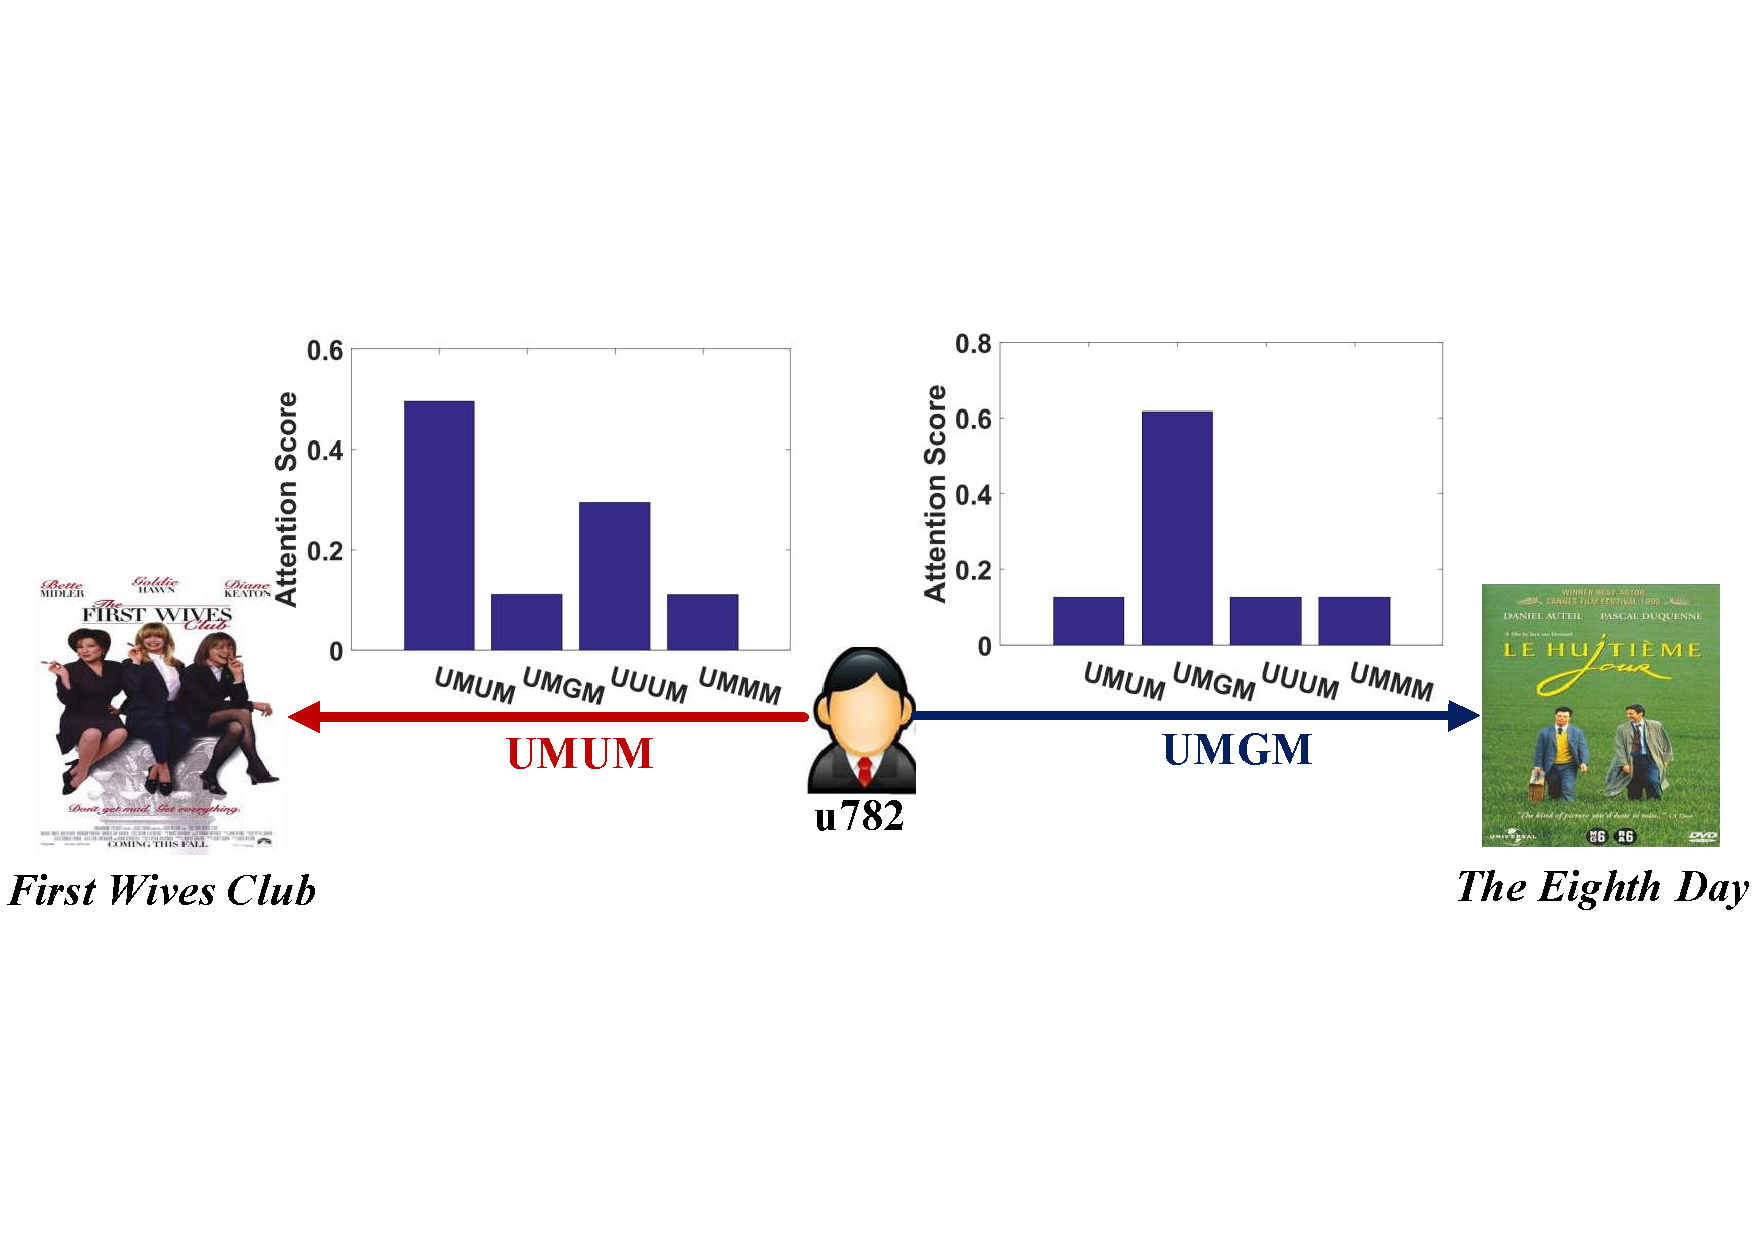
\includegraphics[width=8.5cm]{image/cs_782_2.pdf}\\
  \caption{An illustrative example of the interpretability of interaction-specific attention distributions for MCRec.  \label{fig-casestudy}}
\end{figure}


To see this, we select the user $u782$ in the Movielens dataset as an illustrative example. Two interaction records of  this user have been used here, namely movies of ``\emph{First Wives Club}'' and ``\emph{The Eighth Day}''. In Fig.~\ref{fig-casestudy}, we can see that each interaction corresponds to a unique attention distribution, summarizing the contributions of the meta-paths. The first interaction mainly relies on the meta-paths of $UMUM$ and $UUUM$, while the second interaction mainly relies on the meta-path of $UMGM$. By inspecting into the dataset, it is found that at least five friends of $u782$ have watched the movie of ``\emph{First Wives Club}'', which explains why user-oriented meta-paths  $UMUM$ and $UUUM$ play the key role in the first interaction. As for the second interaction, we find that the movie of ``\emph{The Eighth Day}'' is with the genre of \emph{Drama}, which is the favorite movie genre of $u782$. This explains why genre-oriented meta-path $UMGM$ plays the key role in the second interaction.
Our model is able to produce interaction-specific attention distributions, providing a good interpretability for the recommendation results.

%Furthermore, we investigate the attention scores and recommendations of a concrete user. We select the user $u782$ in the Movielens dataset, and report the distribution of attention scores of this user and the movies recommended in the Fig.~\ref{fig-casestudy}. When recommending the movie ``The Eighth Day'', we find the meta-path $UMGM$ plays the leading role. When we analyze the view records of this user, we can find the favorite of this user are genre Drama, Comedy and Thriller, and the recommended movie ``The Eighth Day'' is just Drama. Meanwhile, the meta-path $UMUM$ is more important when recommending the movie ``First Wives Club''. A potential reason is that the movie ``First Wives Club'' is often watched by users having the same viewing records with the user $u782$, that is the truth after we analyzed the data.  The above analysis reflects that the attention scores of meta-paths effectively reveal users' preferences and the path semantics are potential for explanation recommendation.

After examining how the co-attention works at the user level, we further present the macro-level analysis of the attention distributions for the entire dataset.
We present the box-plot figure of the attention weight distributions from all the interaction records of a dataset in Fig.~\ref{fig-attention-distribution}.
We can see that  the distributions of attention weights are indeed very skew,  indicating some meta-paths are more important to consider than the others.
%In this section, we study the reasonability and physical meaning of meta-paths' attention scores discovered by MCRec. We first make a statistics on the attention scores in the above experiments, and report the distribution of these attention scores in Fig.~\ref{fig-attention-distribution}. As shown in Fig.~\ref{fig-attention-distribution}, we can find that users in the Movielens dataset prefer the meta-path $UMGM$, while users in the Yelp dataset prefer the meta-path $UBCaB$ and $UBCiB$. However, in the LastFM dataset, the distribution of attention scores on each meta-path is quite close. It reveals that the meta-paths in the LastFM dataset have similar contribution on recommendation.  We think it is also the reason why the performance improvement of MCRec against MCRec$_avg$ is not much significant in the Table~\ref{tab_Effectiveness}.

\begin{figure*}[htbp]
\centering
\subfigure[Movielens]{
\begin{minipage}[t]{0.3\linewidth}
\centering
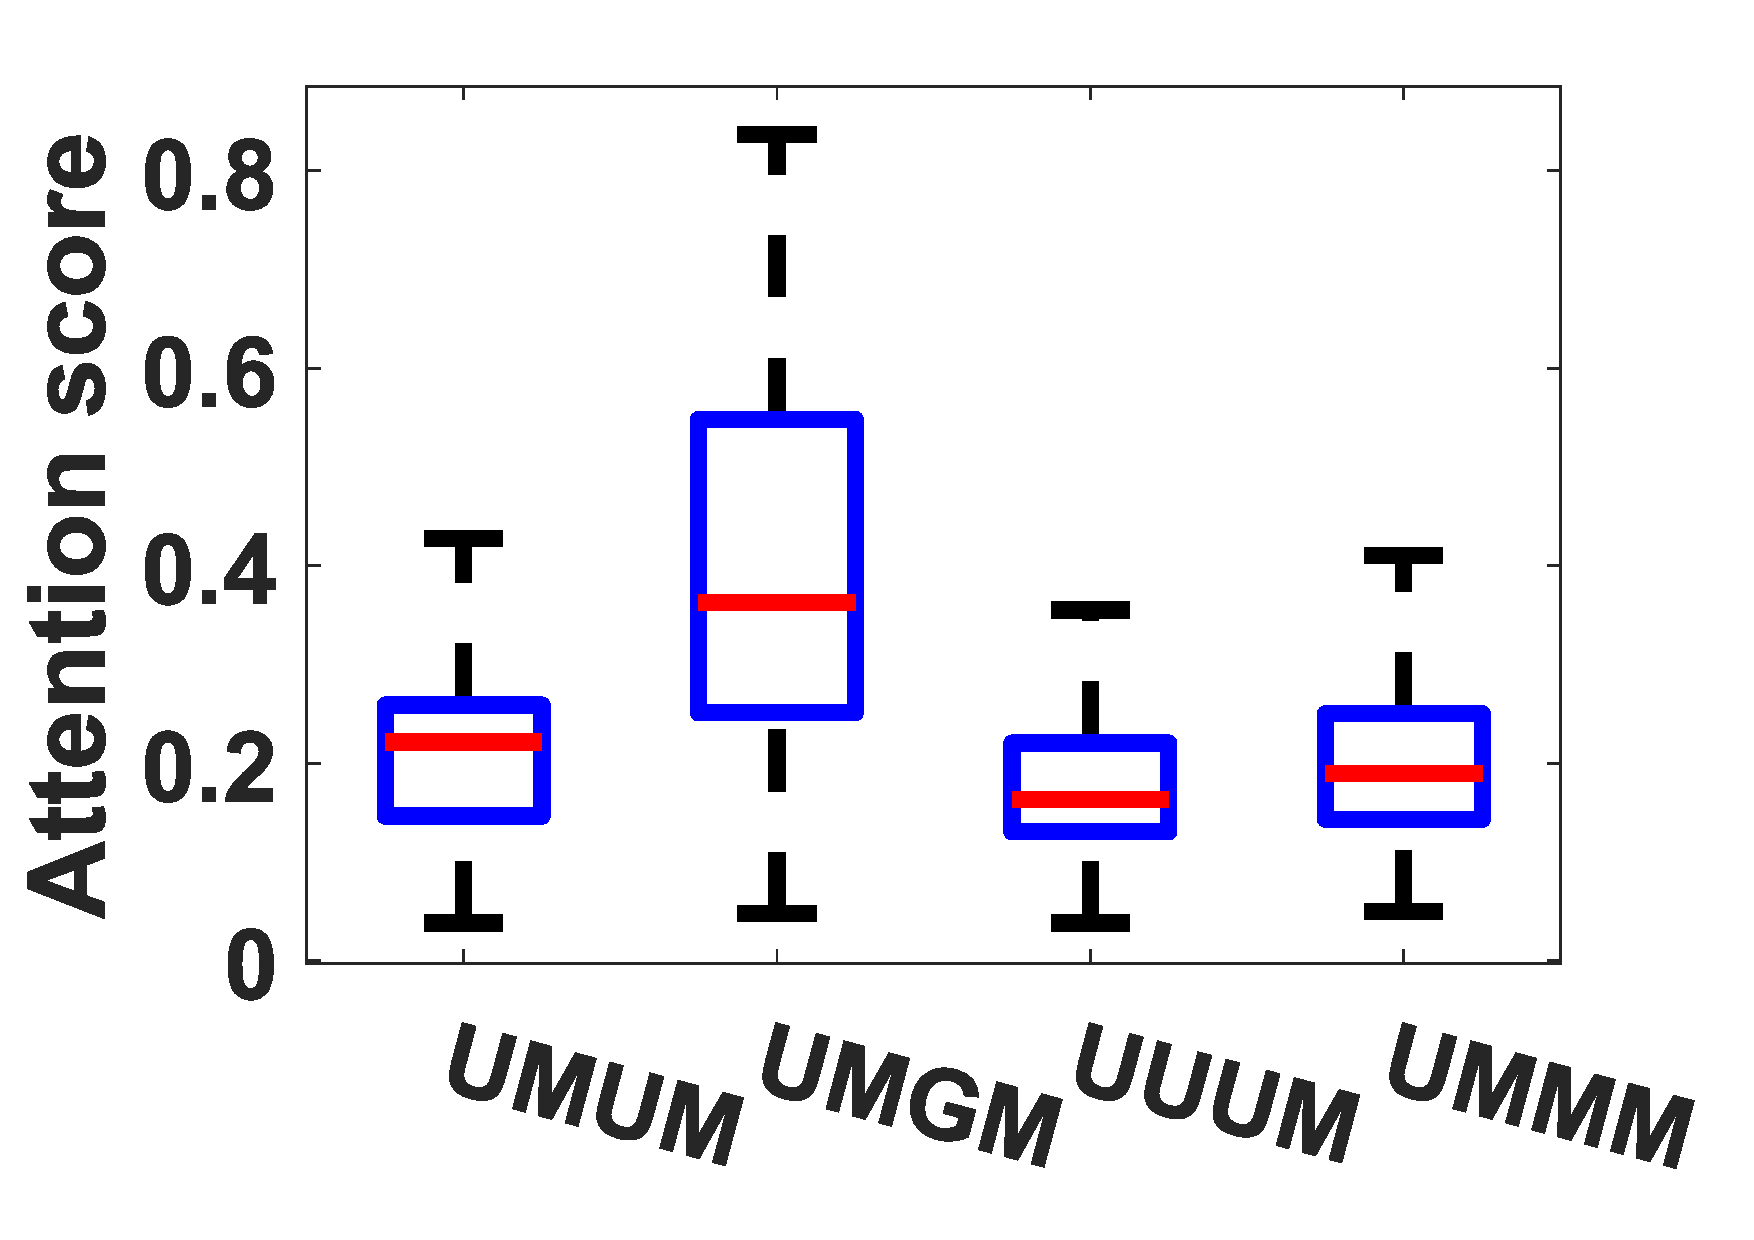
\includegraphics[width=4.2cm]{image/ml_attention_box.pdf} %2.8
\end{minipage}
}
\subfigure[LastFM]{
\begin{minipage}[t]{0.3\linewidth}
\centering
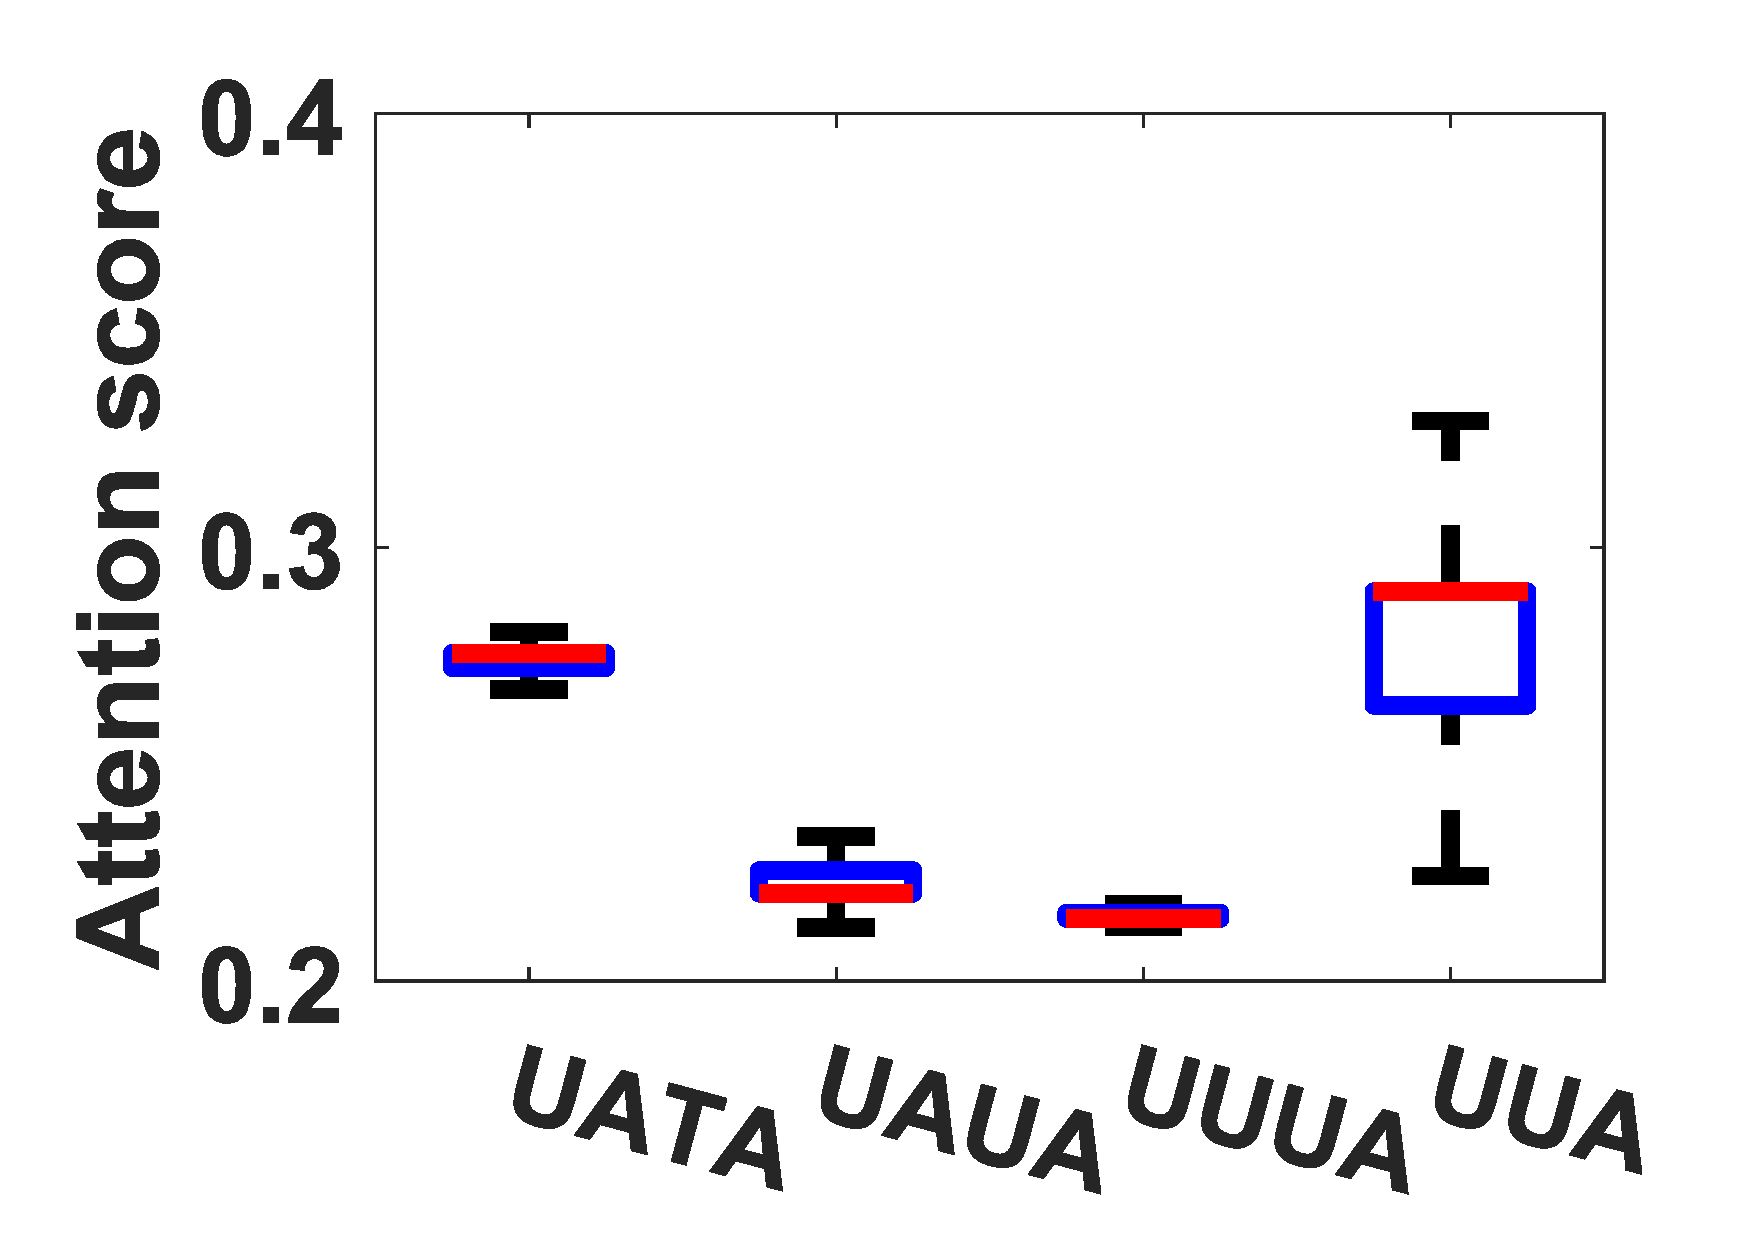
\includegraphics[width=4cm]{image/lm_attention_box.pdf} %2.6
\end{minipage}
}
\subfigure[Yelp]{
\begin{minipage}[t]{0.3\linewidth}
\centering
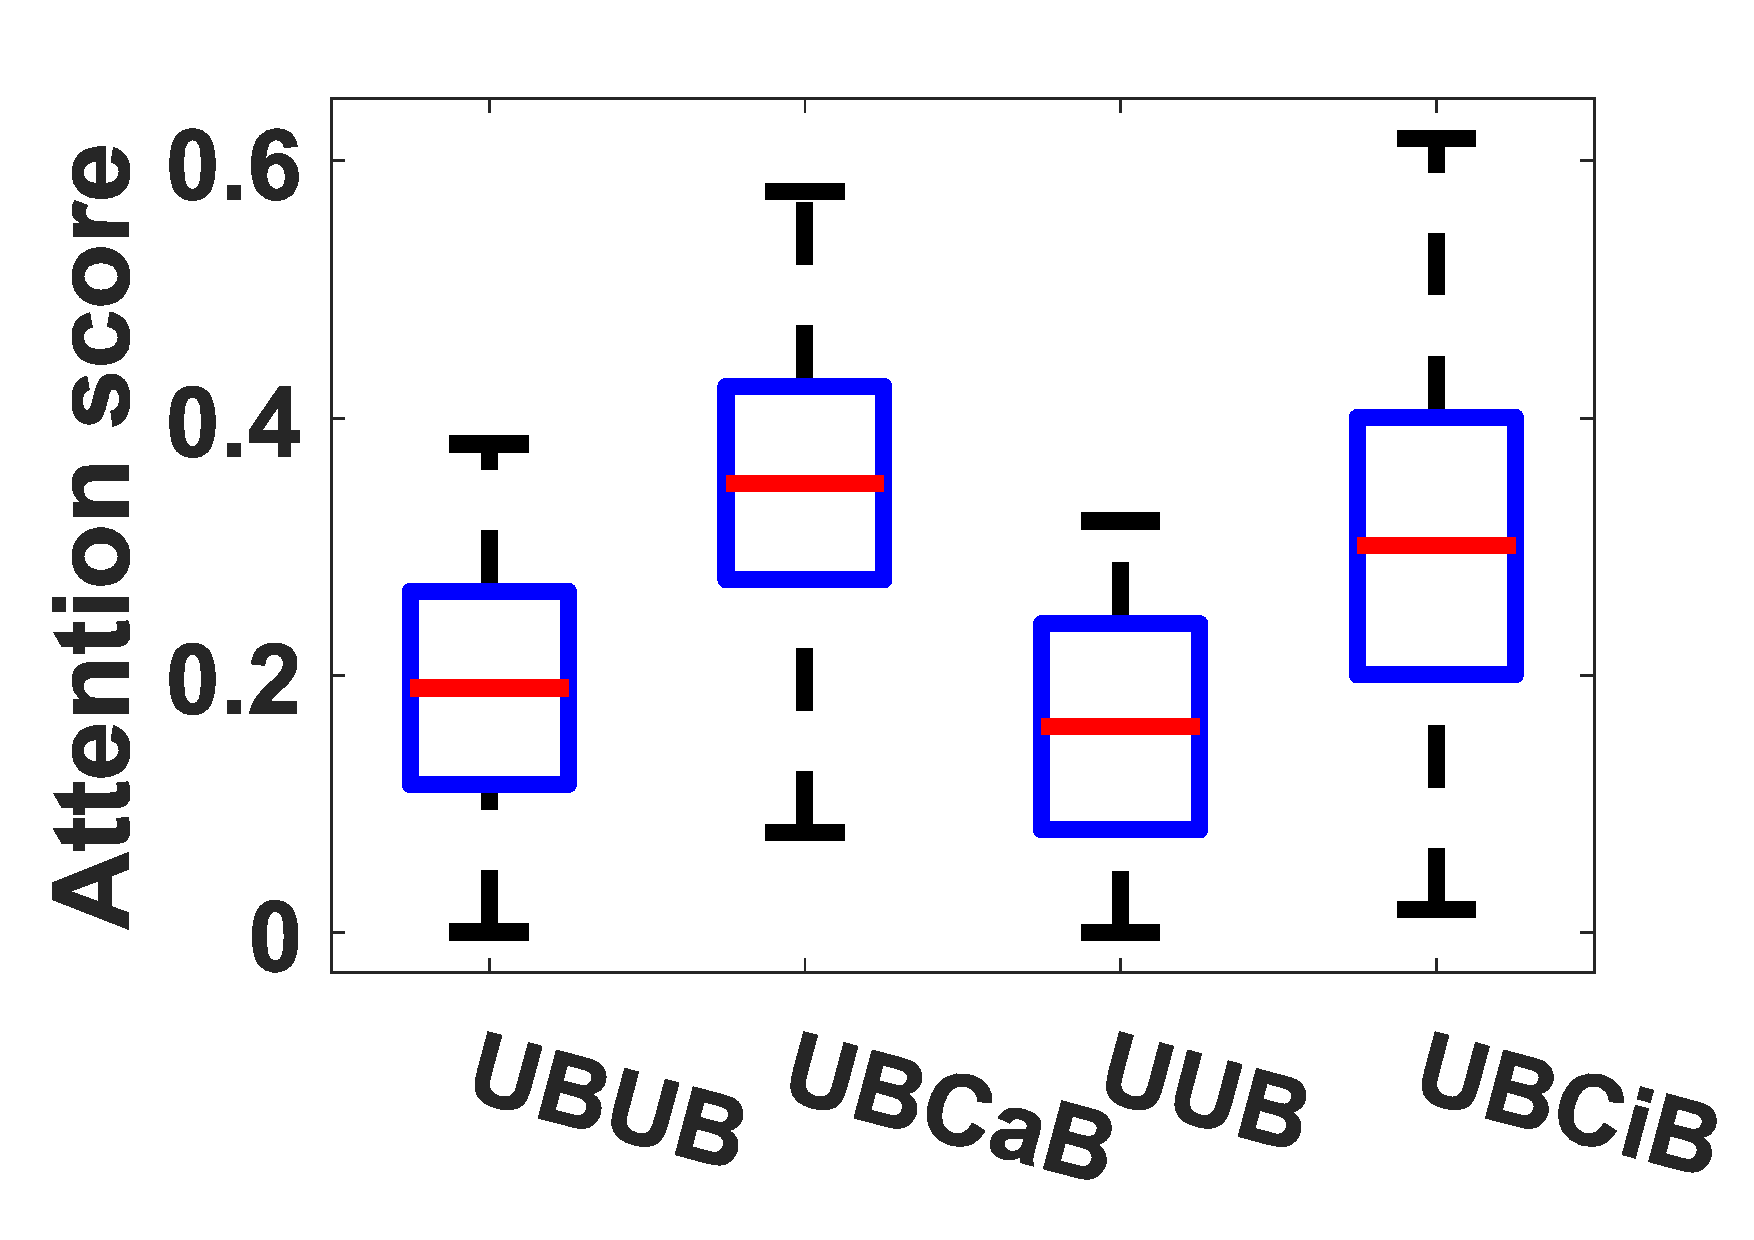
\includegraphics[width=4.2cm]{image/yelp_attention_box.pdf} %2.8
\end{minipage}
}
\caption{The distribution of attention weights of MCRec on the three datasets. \label{fig-attention-distribution}}
\end{figure*}


\subsubsection{Cold-start Recommendation}
HINs are particularly useful to alleviate  cold-start problem in recommendation, where there are very few rating records but heterogeneous context
information is available. We study the recommendation performance \wrt different cold-start degrees, \ie the feedback sparsity.
We divide the entire dataset into five equal folds. The last fold is held out for test, and then we vary the amount of training data from one fold to four folds, corresponding to 20\%, 40\%, 60\%, 80\% data as training sets.  For comparison, we select three representative baselines: BPR, NeuMF, FMG$_{rank}$.
For convenience, we report the improvement ratios \wrt BPR by other comparison methods. Due to space limit, for the remainder of the paper, we will only show the results from Movielens and Yelp, since LastFM shows similar findings. 
As shown in Fig.~\ref{fig-coldstart}, we can see that MCRec yields the most improvement over BPR in all the cases. Overall, the improvement ratios decrease with the increasing of training data. The results indicate that HIN based information is effective to improve the recommendation performance, and the proposed MCRec method can effectively utilize heterogeneous information in a more principled way.


%We present the performance comparison of different methods in Fig.~\ref{fig-coldstart}. For convenience, we report the improvement ratios \wrt BPR. Overall, most of the comparison methods are better than BPR (\eg a positive y-axis value). The proposed method performs the best among all the methods, and the improvement over BPR becomes more significant for users with fewer rating records. The results indicate that HIN-based information is effective to improve the recommendation performance, and the proposed MCRec method can effectively utilize heterogeneous information in a more principled way.

\begin{figure}[htbp]
\centering
\subfigure[Movielens]{
\begin{minipage}[t]{0.45\linewidth}
\centering
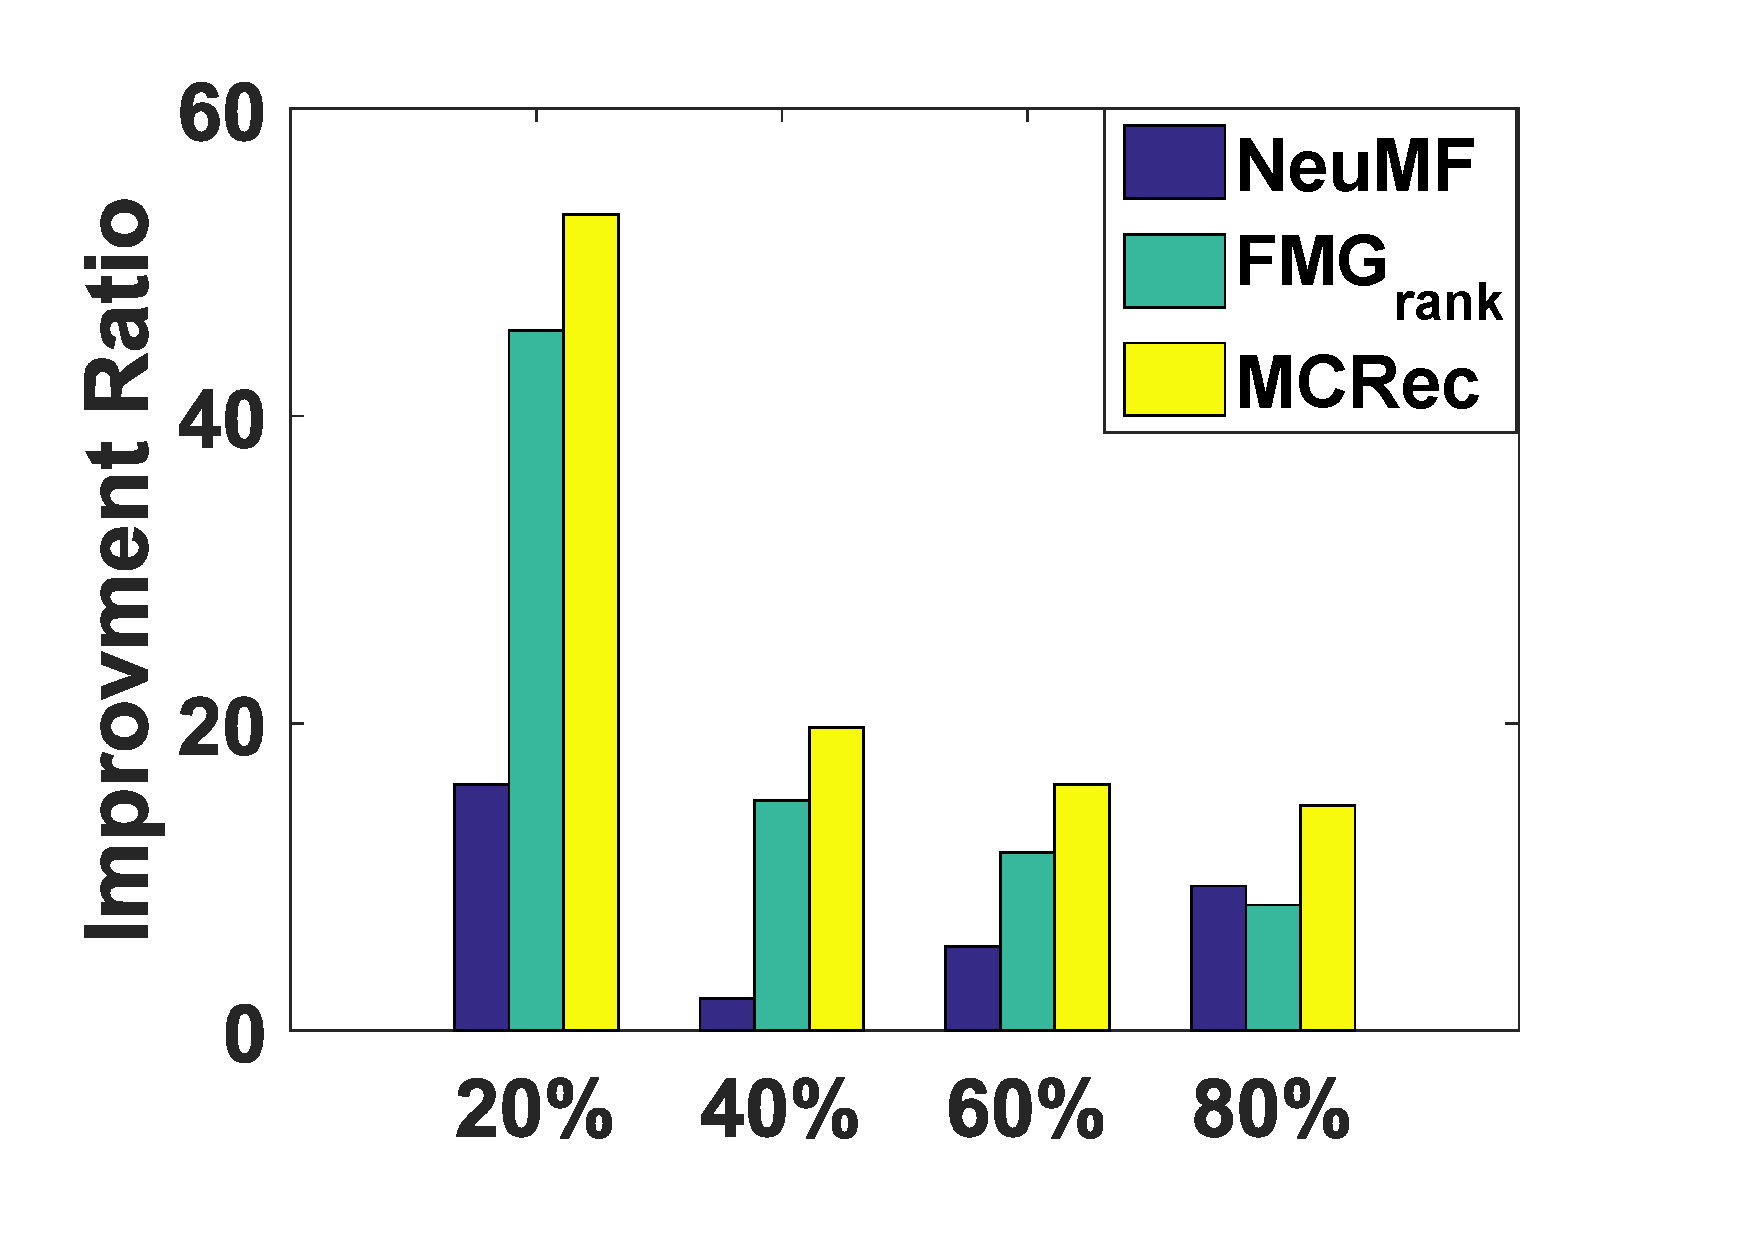
\includegraphics[width=4.4cm]{image/ml_coldstart.pdf}
\end{minipage}
}
%\hspace{30pt}
\subfigure[Yelp]{
\begin{minipage}[t]{0.45\linewidth}
\centering
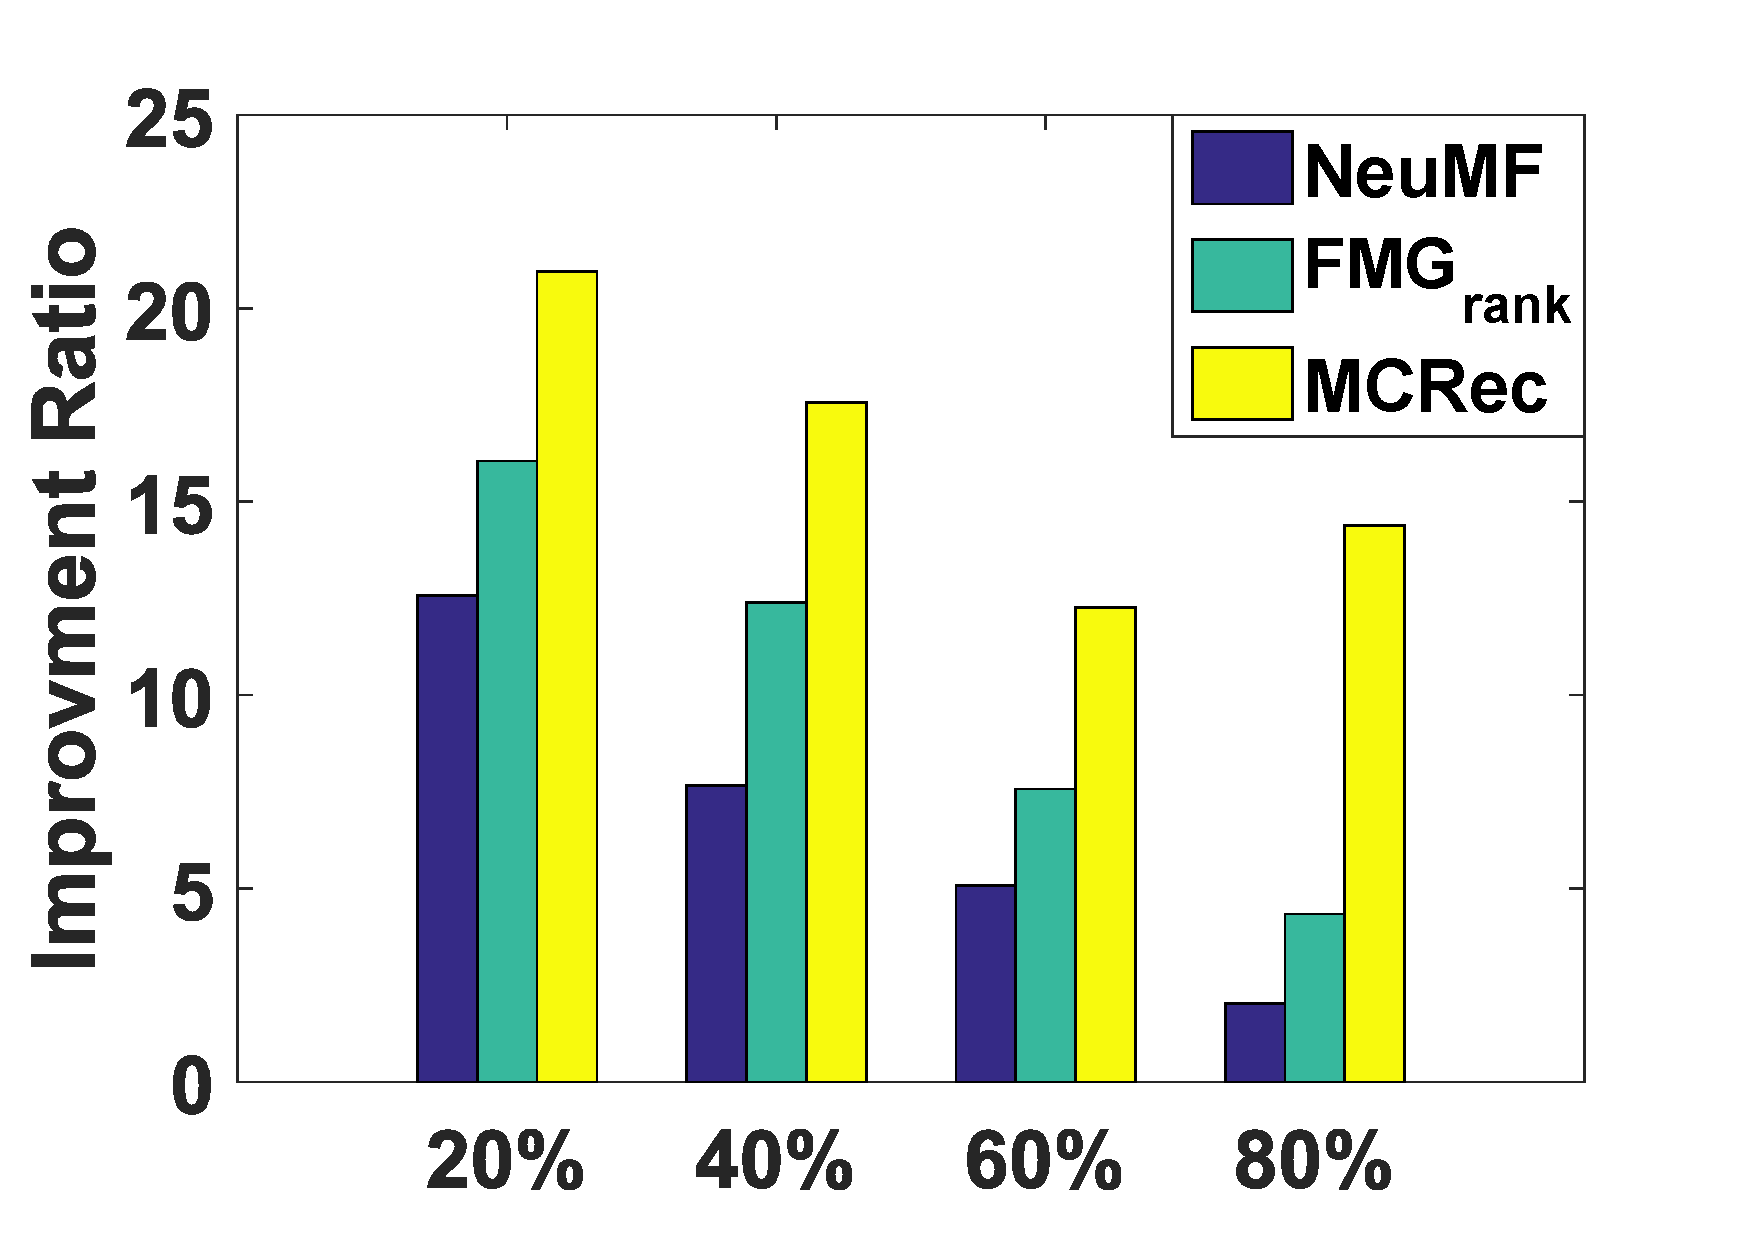
\includegraphics[width=4.3cm]{image/yelp_coldstart.pdf}
\end{minipage}
}
\caption{Performance comparison of different methods for cold-start recommendation on Movielens and Yelp datasets. $y$-axis denotes the improvement ratio over BPR for $Prec@10$.\label{fig-coldstart}}
\end{figure}



\subsubsection{Impact of Different Meta-Paths}
In this section, we analyze the impact of different meta-paths on the recommendation performance through gradually incorporating meta-paths into the proposed model. For ease of analysis, we include the NeuMF as the reference baseline. In Fig.~\ref{fig-meta-path}, we can observe that  the performance of MCRec overall improves with the incorporation of more meta-paths. Meanwhile, meta-paths seem to have different effects on the recommendation performance. Particularly, we can find that, when adding $UMGM$, MCRec has a significantly performance boost in Movielens dataset, while adding $UBCaB$ and $UBCiB$ is more important for Yelp dataset. These findings are consistent with previous observations for attention weights distributions of meta-paths in Fig.~\ref{fig-attention-distribution}, where these meta-paths have higher attention scores.
%We think the reason lies in that these meta-paths contain more useful information for recommendations. Furthermore, we think the same reason makes these meta-paths have larger attention scores in Figure~\ref{fig-attention-distribution}.

\begin{figure}[htbp]
\centering
\subfigure[Movielens]{
\begin{minipage}[t]{0.45\linewidth}
%\centering
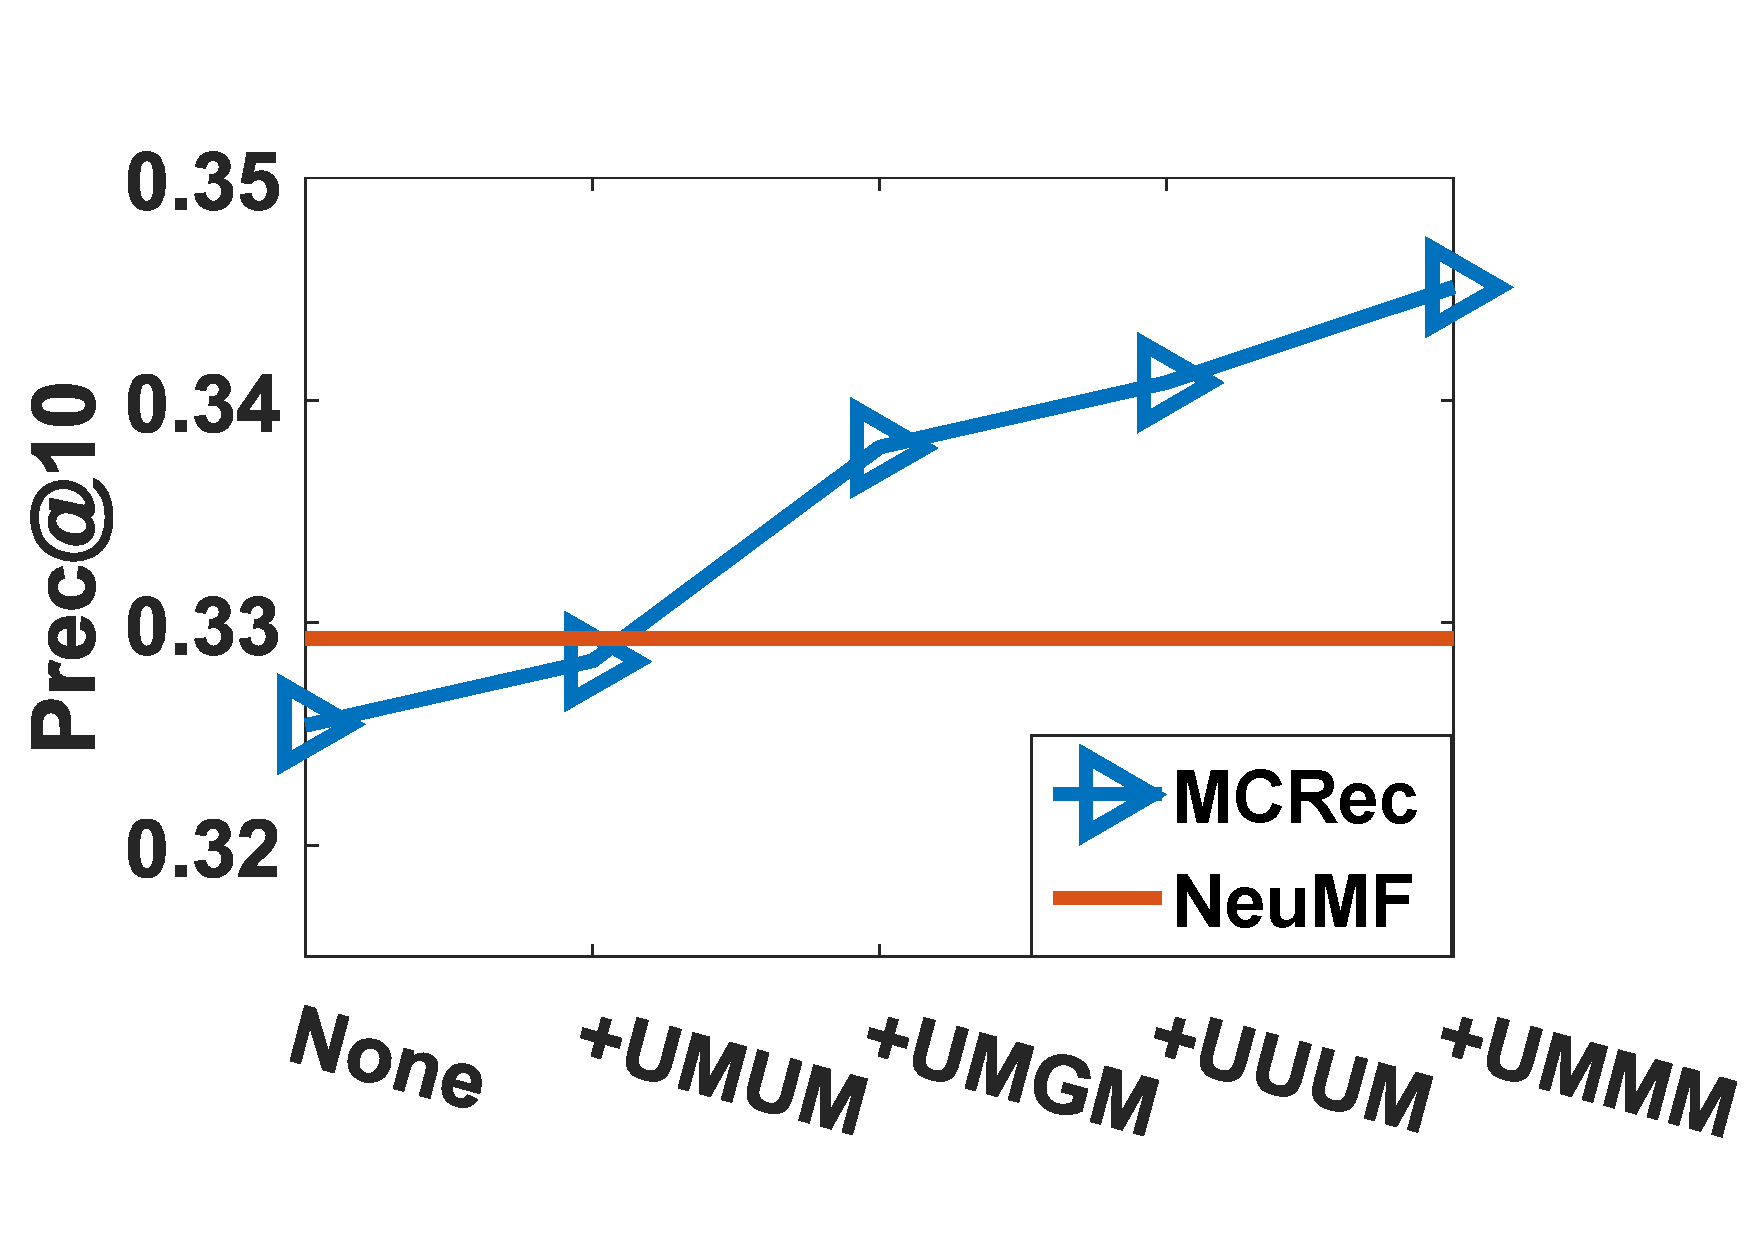
\includegraphics[width=4.15cm]{image/ml_metapath_p.pdf}
\end{minipage}
}
%\hspace{40pt}
\subfigure[Yelp]{
\begin{minipage}[t]{0.45\linewidth}
\centering
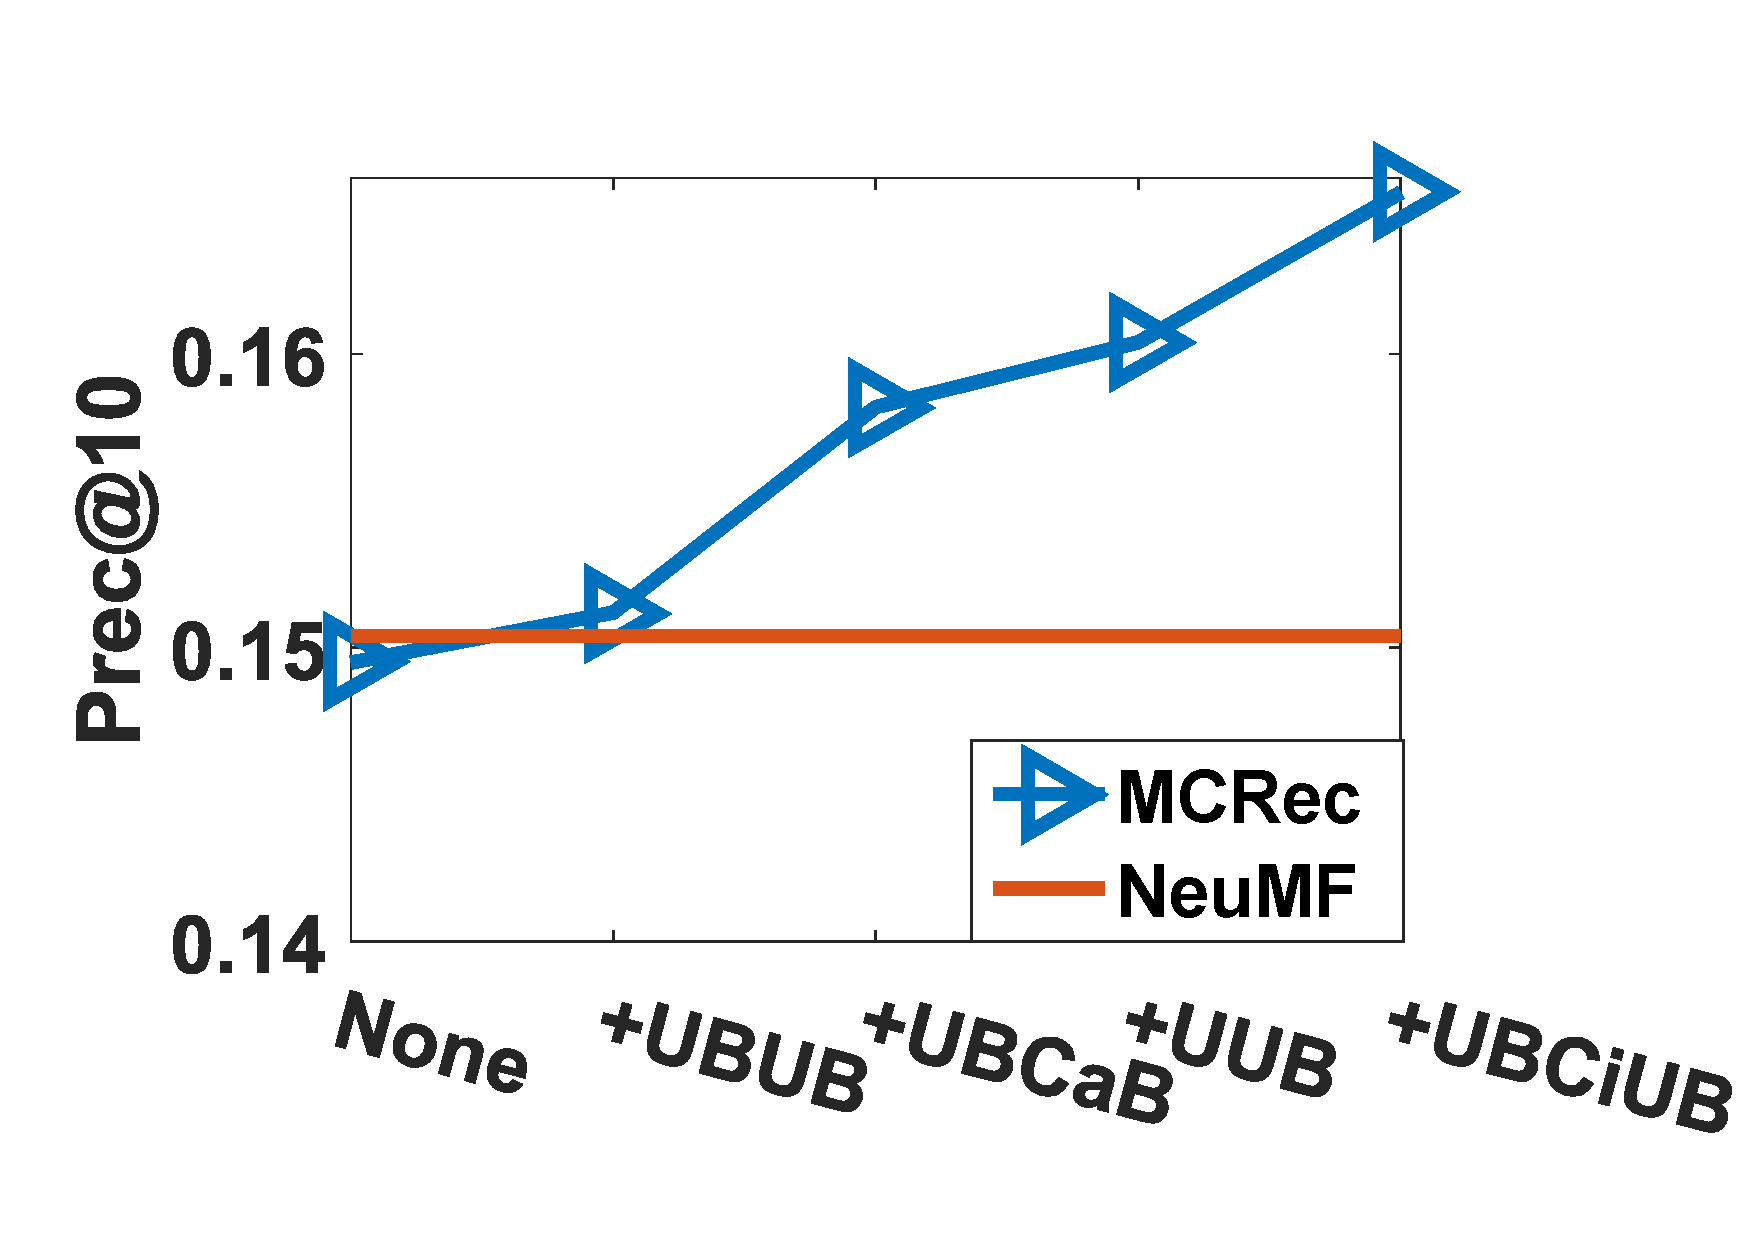
\includegraphics[width=4.2cm]{image/yelp_metapath_p.pdf}
\end{minipage}
}
\caption{Performance change of MCRec when gradually incorporating meta-paths.\label{fig-meta-path}}
\end{figure}


%\subsubsection{Impact of Path Sampling Strategy}
%In Section 4.3.1, we present an importance-based random walk strategy based on meta-path in MCRec. We use the pretrain technique with Factorization Machine to select path instances with higher importance scores. Here, we examine the effectiveness of the propose path sampling strategy.
%In Fig.~\ref{fig-sample}, we can see that the proposed sampling strategy is consistently better than the previous random sampling method.
%With the pretrain latent factors for computing the importance scores, our sampling strategy is able to discover more high-quality path instances for recommendation.

%In order to furtherly validate the effectiveness of  the preference-guided random walk strategy based on meta-path in MCRec, we compare our strategy with traditional path-based random walk strategy widely used in HIN embedding. The results are shown in Fig.~\ref{fig-sample}. We can find the proposed sample strategy significantly  outperforms the traditional strategy. An possible reason is that  the proposed preference-guided walk strategy can sample high-quality path instances, while traditional walk strategy may introduce much noise.
%\begin{figure}[htbp]
%\centering
%\subfigure[Movielens]{
%\begin{minipage}[t]{0.45\linewidth}
%\centering
%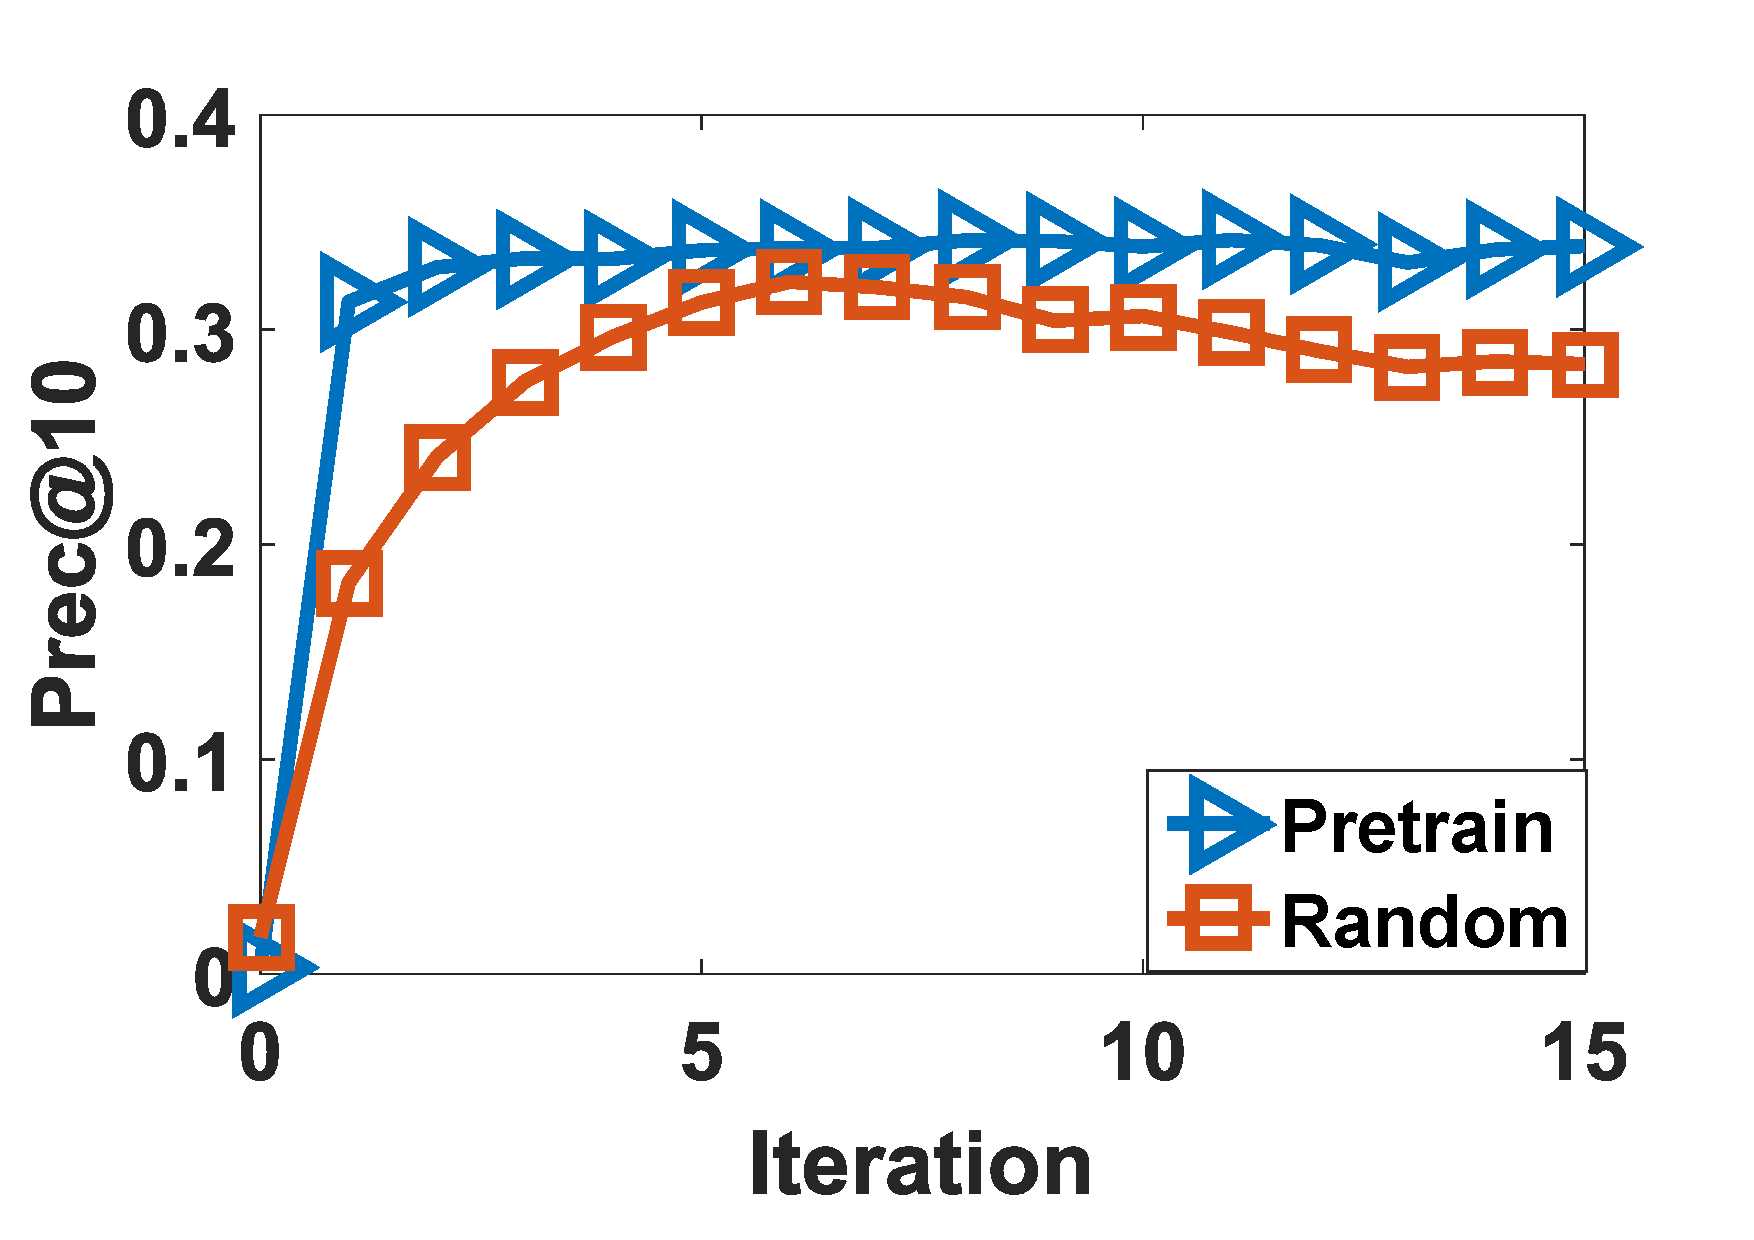
\includegraphics[width=4.2cm]{image/ml_sample_p.pdf}
%\end{minipage}
%}
%\hspace{40pt}
%\subfigure[Yelp]{
%\begin{minipage}[t]{0.45\linewidth}
%\centering
%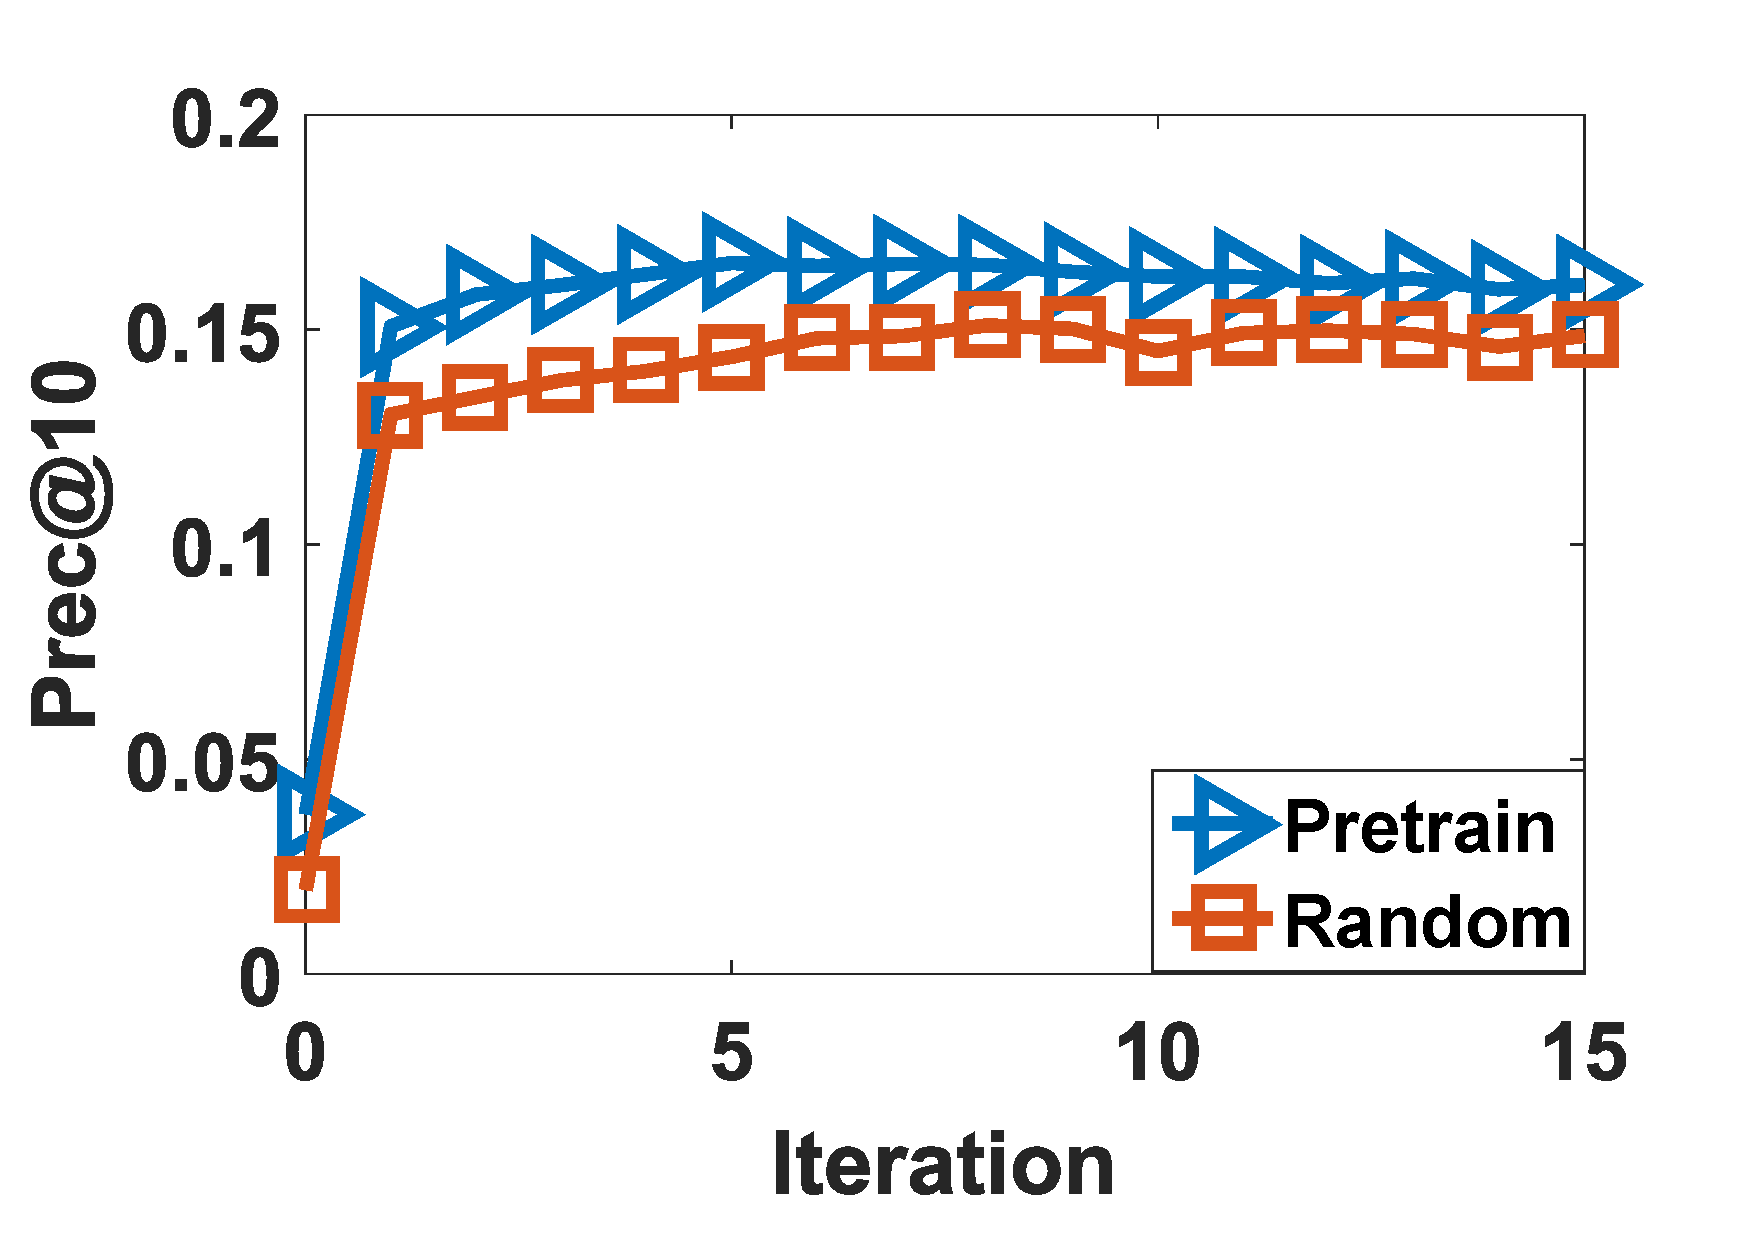
\includegraphics[width=4.2cm]{image/yelp_sample_p.pdf}
%\end{minipage}
%}
%\caption{ Performance with respect to different sampling strategies on Movielens and Yelp datasets.\label{fig-sample}}
%\end{figure}


\subsubsection{Parameter Tuning} Our models include a few important parameters to tune. Here, we examine the performance effect of two parameters, \ie the number of predictive factors (the embedding size for the output layer) and the number of negative samples (in Eq.~\ref{equ-loss}).
For the number of predictive factors, we vary it in the set of \{8, 16, 32, 64\}. For the number of negative samples, we vary it in the set of \{1, 3, 5, 7, 9\}.
As shown in Fig.~\ref{fig-param}, overall MCRec is not sensitive to these two parameters. The optimal performance is obtained with 32 predictive factors and five negative samples.

%near 32. As shown in Fig.~\ref{fig-param}, the optimal performance is around 5.

%In this section, we study two tuning parameters involved in our prediction model, which are the predictive factors and the number of negative samples. Now we check how they influence the model performance. Due to space limitation, we just present the results
%on Movielens dataset.

\begin{figure}[htbp]
\centering
\subfigure[\#predictive factors]{
\begin{minipage}[t]{0.45\linewidth}
\centering
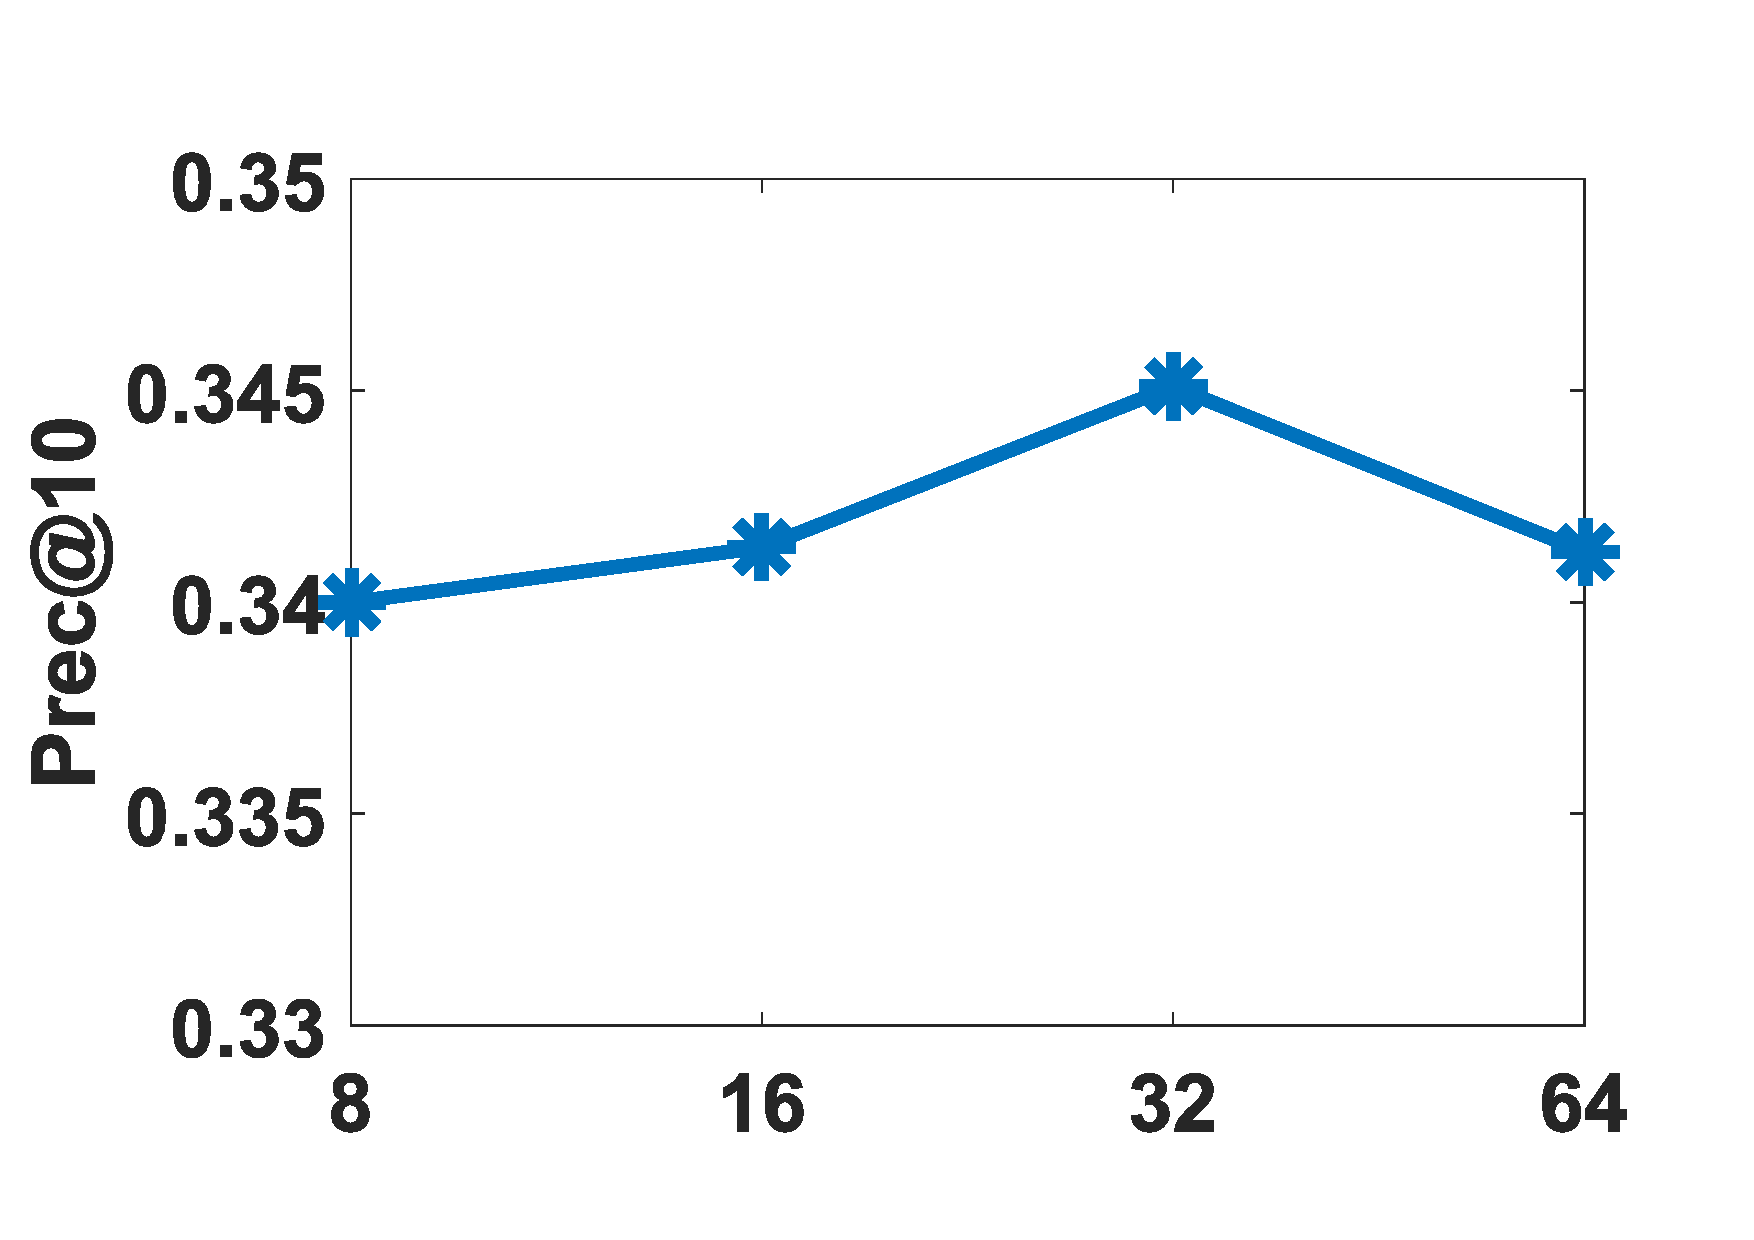
\includegraphics[width=4.2cm]{image/ml_factors_p.pdf}
\end{minipage}
}
%\hspace{40pt}
\subfigure[\#negative samples]{
\begin{minipage}[t]{0.45\linewidth}
\centering
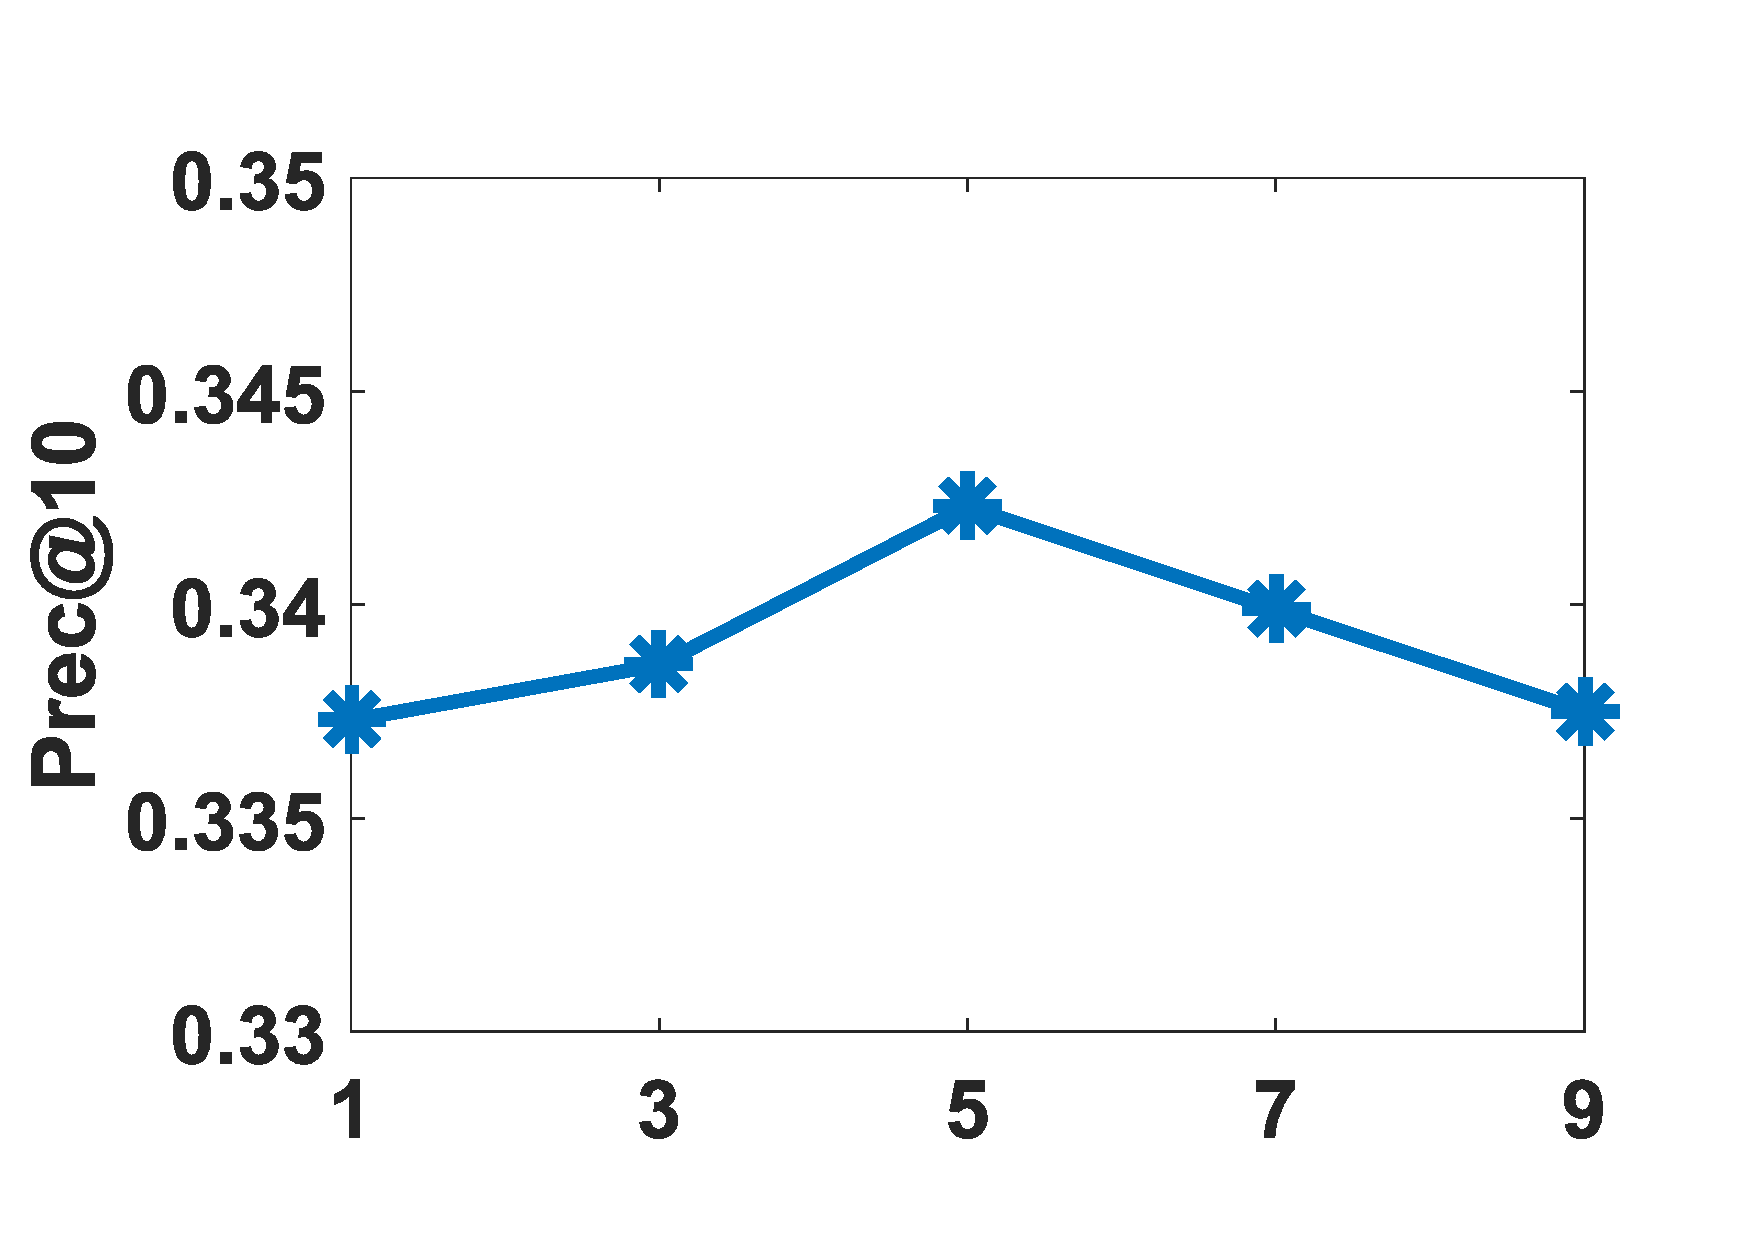
\includegraphics[width=4.2cm]{image/ml_negative_p.pdf}
\end{minipage}
}
\caption{Parameter tuning of MCRec on Movielens dataset.\label{fig-param}}
\end{figure}














